%%%%%%%%%%%%%%%%%%%%%%%%%%%%%%%%%%%%%%%%%%%%%%%%%%%%%%%%%%%%%%%%%%%%%%%%%%%%%%%%%%%%%%%%%%%%%
%%									Chapitre 6												%
%%%%%%%%%%%%%%%%%%%%%%%%%%%%%%%%%%%%%%%%%%%%%%%%%%%%%%%%%%%%%%%%%%%%%%%%%%%%%%%%%%%%%%%%%%%%%

\chapter{Cartographie quantitative de susceptibilité magnétique}
\label{chap:qsm}
	\minitoc

%%%%%%%%%%%%%%%%%%%%%%%%%%%%%%%%%%%%%%%%%%%%%%%%%%%%%%%%%%%%%%%%%%%%%%%%%%%%%%%%%%%%%%%%%%%%%


L’imagerie quantitative de susceptibilité magnétique est une technique récente permettant
d’évaluer quantitativement la susceptibilité des structures dans le cerveau. Cette imagerie est encore
en développement, il existe de nombreux algorithmes différents permettant de résoudre les différents
problèmes rencontrés lors de la reconstruction d’une QSM. Il est donc indispensable de sélectionner
ceux offrant le meilleur résultat au vue du matériel utilisé. Dans le cadre de cette thèse, l’ensemble
des acquisitions ont été réalisées sur une IRM Siemens Skyra à 3T (Skyra, Siemens, Allemagne).

Nous aborderons tout d’abord les méthodes permettant de mettre en place la chaîne de
reconstruction et les implémentations réalisées permettant d’aboutir à une mesure correcte de la
susceptibilité. Par la suite nous décrirons les méthodes de validation de cette mesure de susceptibilité.
En effet, comme avec toute nouvelle méthode de reconstruction IRM, il est indispensable d’effectuer
un contrôle qualité permettant de valider la mesure.
%%%
%%%
%%%
\section{Théorie}
%%%
%%%
\subsection{Principe}
Pour comprendre le principe de construction d’une carte de susceptibilité, il est nécessaire de
revenir sur quelques équations importantes permettant de remonter de la phase à la susceptibilité.

La première étape est d’obtenir la cartographie de perturbation du champ à partir de l’image
de phase. Une relation directe existe entre cette cartographie et la phase via l’équation suivante (\cite{Bilgic2012}):
\begin{equation}
\label{eq:champ_phase}
B\,=\,\frac{\phi}{B_0\,\gamma\,T_E}.
\end{equation}
Dans cette équation, $B$ est carte de perturbation du champ normalisée, $\phi$ est la phase
mesurée, $B_0 $ la force du champ magnétique extérieur appliqué (en Tesla), $\gamma$ est le rapport
gyromagnétique du proton et $T_E$ le temps d’écho. Précisons que la perturbation du champ $B$
correspond à :
\begin{equation}
B_{total}\,=\,B_0\,+\,B.
\end{equation}
Les équations de la magnétostatique de Maxwell, fournissent alors, dans l’espace réciproque
une relation entre la perturbation du champ $B $ et la distribution de susceptibilité:
\begin{equation}
{\cal F}\,B\,=\,\biggl(\frac{1}{3}-\frac{k_z^2}{k_x^2+k_y^2+k_z^2}\biggr)\,\circ\,({\cal F}\chi )
\end{equation}
où ${\cal F}$ la transformée de Fourier, $k_x$ , $k_y$ et $k_z$ sont les coordonnées du vecteur d’ondes, la direction $Z$
coincidant avec celle du champ $B_0$.\\
Notez qu’on peut simplifier cette expression en définissant le kernel D qui relie la carte de champ à la
susceptibilité :
\begin{eqnarray}
{\cal D}\,=\,\biggl(\frac{1}{3}-\frac{k_z^2}{k_x^2+k_y^2+k_z^2}\biggr)\\
\chi\,=\,{\cal F}^{-1}\,{\cal D}^{-1}\,{\cal F} B.
\end{eqnarray}
La définition de D, et la singularité de son inverse lorsque
\begin{equation}
\biggl(\frac{1}{3}-\frac{k_z^2}{k_x^2+k_y^2+k_z^2}\biggr)\,=\,0
\end{equation}
met en évidence le caractère mal posé du problème.

Ces notions de bases en susceptbilité magnétique permettent d’appréhender le passage de
l’image de phase à une image quantitative de susceptibilité magnétique. On distingue donc différentes
étapes : l’acquisition, l’obtention d’une phase cohérente, le passage à la carte de perturbation du
champ, et l’inversion finale aboutissant à la cartographie de susceptibilité (Figure~\ref{fig:6_1_carte_susceptibilite}).
%%%
\begin{figure}[!t]
\centering
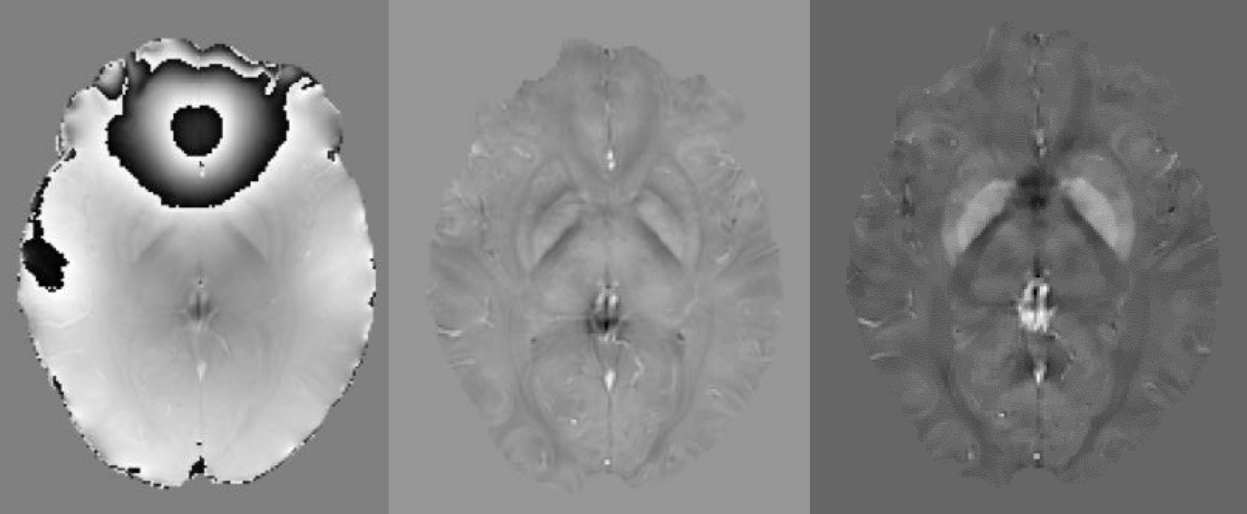
\includegraphics[width=12cm]{6_1_carte_susceptibilite}
\caption{Exemple de carte de susceptibilité magnétique. De gauche à droite, l'image de phase, la carte de perturbation
de champ intérieur, et la carte de susceptibilité magnétique reconstruite.}
\label{fig:6_1_carte_susceptibilite}	
\end{figure}
%%%
\subsection{Un ou plusieurs temps d'échos?}
L’acquisition est réalisée via une séquence en écho de gradient standard, ou une séquence
dédiée avec compensation de flux dans les 3 directions ({\cite{Deistung2009}). En fonction des objectifs et du temps
machine disponible selon l’étude pour réaliser l’acquisition, deux approches ont été développées.
L’une au cours de laquelle plusieurs échos sont acquis à différents moments après l’impulsion
radiofréquence (approche multi-T$_E$), et l’autre ou un seul temps d’écho est utilisé (simple-T$_E$).

Quels sont les avantages d’une acquisition à un ou plusieurs temps d’échos ?

L’avantage principal de l’acquisiton simple-T$_E$ est la brieveté de la séquence correspondance (4
minutes) au lieu de 8 minutes environ pour des séquences multi-T$_E$ (8 TE). Néanmoins en terme de
qualité de la reconstruction la séquence multi-T$_E$ présente d’importants avantages.

En effet, l’image de phase est codée entre $-\pi$ et $+\pi$. Lorsque le déphasage est supérieur à $2\pi$,
un artefact du signal de phase apparait, appelé saut de phase ou repliement de phase. En effet,
considérons l’échelle de codage des intensités comme un cercle dont $0$ est le minimum et $2\pi$ le
maximum : lorsque le déphasage dépasse $2\pi$, la valeur stockée sera la valeur suivante sur l’échelle,
c’est-à-dire $0$. Il faut alors {\em déplier} la phase (Figure~\ref{fig:6_2_depliement}). Or une image de phase comporte en général un grand nombre de repliements du fait des fortes susceptibilités des interfaces air – tissu et air – crâne
ayant des effets non locaux. Comme le montre la Figure~\ref{fig:6_2_depliement} à une dimension le dépliement de phase
est un problème simple. Cependant à deux et trois dimensions le problème est rendu plus difficile car
nous n’avons plus à faire à des points de dépliements mais à des contours qui se manifestent soit sous
forme de boucles fermées dans l’objet soit de lignes qui commencent et se terminent aux bords de
l’objet. L’algorithme de dépliement doit alors identifier la topologie de façon à rendre le dépliement
cohérent. Notons au passage que dans les méthodes les plus simples de type SWI, ce problème n’est
pas résolu : on se contente de filtrer l’image de phase par un simple filtre passe haut avant de multiplier
cette image filtrée par l’image de magnitude. L’information quantitative de la phase perd une grande
partie de sa signification physique.

%%%
\begin{figure}[!t]
\centering
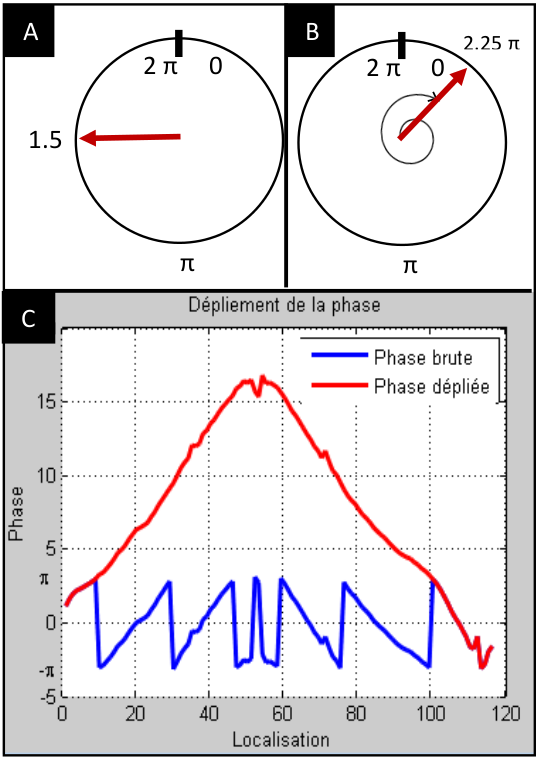
\includegraphics[width=7cm]{6_2_depliement}
\caption{Illustration du dépliement de phase. Sur l’image A, le déphasage observé est de 1.5 $\pi$, donc dans la gamme de valeurs
de l’échelle. Sur l’image B, le déphasage est de 2.25 $\pi$ donc plus grand que les $2\pi$ autorisés, ainsi la valeur récupérée sur
l’image sera de 0.25 $\pi$. La figure C illustre le principe de dépliement de phase, avec en bleu un profil d’une image de phase à
1D et en rouge la même phase dépliée.
}
\label{fig:6_2_depliement}	
\end{figure}
Comme nous allons le voir, en simple T$_E$, les sauts de phases sont plus fréquents et vont donc
requérir l’utilisation d’algorithme de dépliement 3D très robustes, ce qui est le cas des plus récents
(\cite{Schofield2003},~\cite{Witoszynskyj2009}). Si le rapport signal sur bruit est suffisament élevé, une cartographie précise du champ peut
en effet être obtenue par simple écho. On doit supposer alors que la phase est nulle au centre de
l’impulsion radiofréquence (T$_E$=0). Pour un temps d’écho donné, l’écart maximal à la fréquence
centrale est donné par :
\begin{equation}
\omega_{max}\,=\,\frac{\pi}{T_E}.
\end{equation}
Cette formule nous permet de comprendre que lorsque le T$_E$ est petit on a accès à des
fréquences plus importantes ($\omega_{max}$ en radians/sec). Sur l’interval de déphasage $[-\pi,+\pi]$ on observera
moins d’évènements de repliements rendant le traitement plus facile et évitant l’apparition de très
grandes valeurs de la phase en certains points de l’image, source de problèmes dans la reconstruction
du champ intérieur. Mais on sait par ailleurs que le temps d’écho le plus court accessible est limité par
la force du gradient, la résolution et le champ de vue de l’image acquise. Enfin un temps d’écho plus
long est préférable pour améliorer le rapport signal sur bruit. Il faut donc en simple-T$_E$ choisir entre
qualité du signal et facilité du dépliement de phase.

Dans l’approche multi-T$_E$, pour estimer la carte de perturbation du champ, la phase de chaque
voxel le long des temps d’échos est dépliée. Les phases sont ensuites ajustées par méthode des
moindres carrés, et la pente de la courbe est utilisée comme phase de référence (\cite{Kressler2010}). 

Or dans cette approche c’est l’écart inter-écho qui va déterminer la fréquence maximale :
\begin{equation}
\omega_{max}\,=\,\frac{\pi}{\Delta T_E}.
\end{equation}
Ainsi, la fréquence maximale autorisée sera plus grande dans une séquence multi-T$_E$, ce qui se traduit
par moins de repliements de phase et limite les problèmes mentionnés plus haut sans diminution du
rapport signal sur bruit.

Les études récentes ont montrés que les cartes de susceptibilités reconstruites via les
approches simple et multi-échos ne différaient que peu (\cite{Bilgic2012},~\cite{Schweser2012}) au vue des outils de dépliements
de phase maintenant disponibles.

%%%
%%%
\subsection{Reconstruction de la phase}
\label{sec:reconstruction}
Pour envisager de générer une QSM correcte, il faut avant tout s’assurer d’avoir une image de
phase cohérente. Les nouvelles antennes en réseau phasés permettent d’obtenir une qualité d’image
très bonne en un temps réduit. Cependant, l’utilisation d’un tel matériel génère autant d’images qu’il
y a de canaux (20 à 32 en général). Ces images doivent donc être combinées afin d’aboutir à l’image
finale. Il existe deux approches « standard » permettant de faire cela, la méthode SoS pour « Sum Of
Square », et le mode « adaptatif » (\cite{Walsh2000}). Or le problème de ces méthodes est qu’elles sont adaptées à
l’image de magnitude et pas à l’image de phase. Cela engendre l’apparition d’artefacts (Figure~\ref{fig:6_3_artefact_phase}). En
effet, la phase est sujette aux repliements de phase de $2\pi$ dont nous avons parlés, mais qui sont ici
incohérents (discontinuité des sauts). Afin de palier à ce problème, différentes approches ont été
développées. Certaines utilisent les cartes de sensibilité des différents canaux (\cite{Robinson2011}). L’une d’entre elles
utilise une approche de sensibilité unifiée qui incorpore les profils de sensibilités issue d’une
acquisition préalable (\cite{Ros2009}).
%%%
\begin{figure}[!t]
\centering
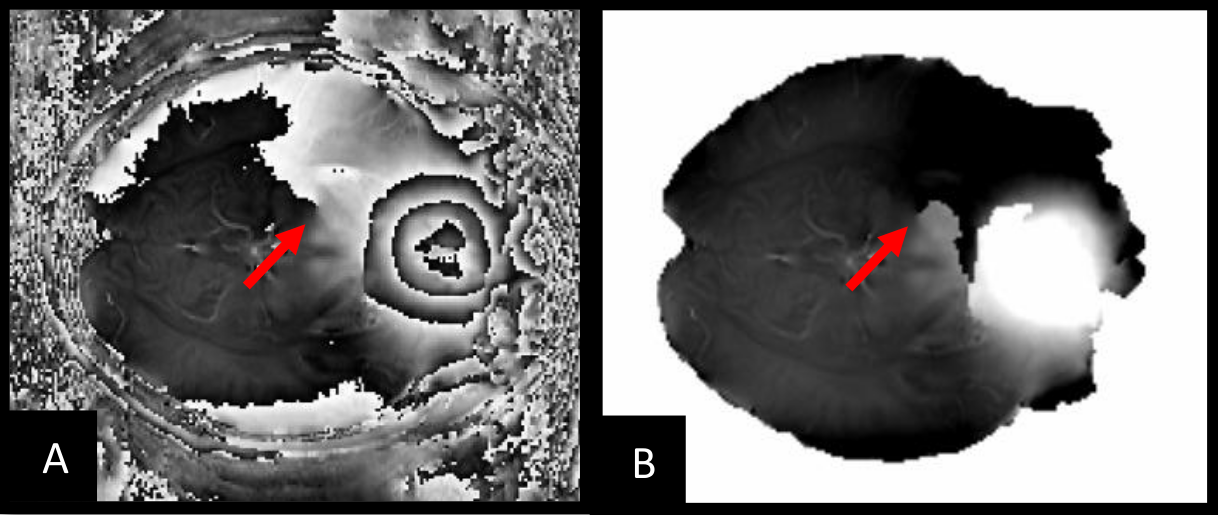
\includegraphics[width=10cm]{6_3_artefact_phase}
\caption{Exemple d'artefact de phase. A) Image de phase après combinaison via le mode adaptatif. La flèche rouge
indique la zone d'incohérence de la phase. B) Image de phase dépliée par un algorithme dédié (PRELUDE), la flèche
rouge indique l'effet de l'artefact vue sur la phase.}
\label{fig:6_3_artefact_phase}	
\end{figure}
Celle-ci est obtenue en réalisant une acquisition basse résolution avec l’antenne corps et l’antenne
multi-canaux. Les images des canaux de l’antenne sont ensuite divisées par l’image de l’antenne corps
pour générer une cartographie brute de sensibilité, sur laquelle sera appliqué un ajustement
polynomial d’ordre variable selon le territoire. On aboutit ainsi à la cartographie finale de sensibilité.
Le signal complexe mesuré dans chaque canal est une pondération du signal « vrai » et de la sensibilité
du canal d’antenne :
\begin{equation}
I_i \,=\,C_i\,\rho,
\end{equation}
où $C$ est la sensibilité par élément d’antenne, $\rho$ le signal « vrai », $i$ le numéro du canal et $I$ la valeur
d’intensité complexe par élément d’antenne.

Disposant d’autant d’équations par voxel qu’il y a de canaux d’antenne, le signal « vrai » peut être
récupéré via une simple inversion matricielle (méthode de Ros et al. - \cite{Ros2009}):
\begin{equation}
\rho\,=\,\bigl(C^H\,\cdot\, C\bigr)\,\cdot\,C^H\,\cdot\,I.
\end{equation}
A partir du signal complexe récupéré, il devient possible d’extraire une magnitude et d’une phase
dépourvue d’artéfacts (Figure~\ref{fig:6_4_ros}). Les sauts de phases sont cohérents, et les artéfacts de discontinuités
au milieu du cerveau disparaissent.

%%%
\begin{figure}[!t]
\centering
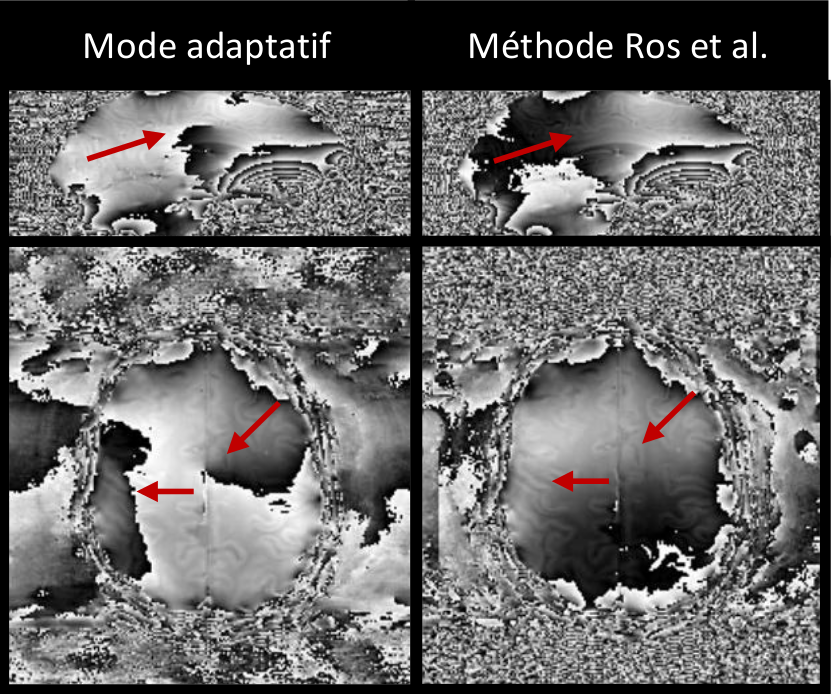
\includegraphics[width=10cm]{6_4_ros}
\caption{Comparaison du mode de combinaison adaptatif (à
gauche) et de la méthode de Ros et al. (à droite). Les flèches
rouges indiquent les zones présentant des artéfacts via la
méthode adaptative.}
\label{fig:6_4_ros}	
\end{figure}
Avant de convertir la phase en carte de perturbation du champ, il est comme on l’a vu
indispensable de la déplier afin de corriger les sauts de $2\pi$. La méthode consiste à prendre un point
de référence et d’utiliser la propriété de continuité spatiotemporelle de la phase, de façon à "recoller"
les valeurs négatives à la valeur positive la plus proche. On a ainsi une phase qui varie de façon continue
plutôt que par paliers. Les approches initiales ne consistaient pas en un « vrai » dépliement, mais comme
pour le SWI en un simple filtre passe haut (\cite{Reichenbach2001}). Ceci avait pour effet de retirer les repliements, mais
aussi des fréquences locales importantes pour certains grands faisceaux de fibres de la matière
blanche. De « vrais » algorithmes de dépliement de la phase sont maintenant disponibles, fonctionnant
soit selon un principe de croissance de région d’intérêt avec identification automatique du point initial
(\cite{Witoszynskyj2009}), soit selon une approche de fusion de régions (FSL PRELUDE) (\cite{Jenkinson2003}), ou encore de sélection du
meilleur chemin (\cite{Abdul-Rahman2007}). Dans ces approches spatiales, le temps de calcul est un élément clef du fait de
la perspective de l’intégration de ces algorithmes dans les outils de reconstruction en ligne. Bien que
certains algorithmes visent à les réduire, ces temps restent non négligeables.
Il existe néanmoins une solution mathématique proposée par Schofield et Zhu en 2003 (\cite{Schofield2003}), qui
présente plusieurs avantages. Il s’agît d’abord d’une solution directe (Équation~\ref{eq:methlaplacien}) rapidement
calculable (avantage en temps de calcul) :
\begin{equation}
\label{eq:methlaplacien}
\theta(k)\,=\,\frac{{\cal F}\{cos\theta {\cal F}^{-1} [k^2{\cal F}(sin\theta)]-sin\theta{\cal F}^{-1}[k^2{\cal F}(cos\theta)]\}}{k^2},
\end{equation}
Où $\theta$ la phase, et $k$ le kernel laplacien.

La méthode est aussi plus performante au niveau de la sensibilité aux artéfacts de phases
(Figure~\ref{fig:6_5_exemples_depliement}) qui malgré les corrections des méthodes de combinaison des canaux d’antennes,
pourraient subvenir. Du fait de sa rapidité et sa fiabilité, cette méthode devient la plus utilisée dans le
domaine de l’imagerie de susceptibilité magnétique.
%%%
\begin{figure}[!t]
\centering
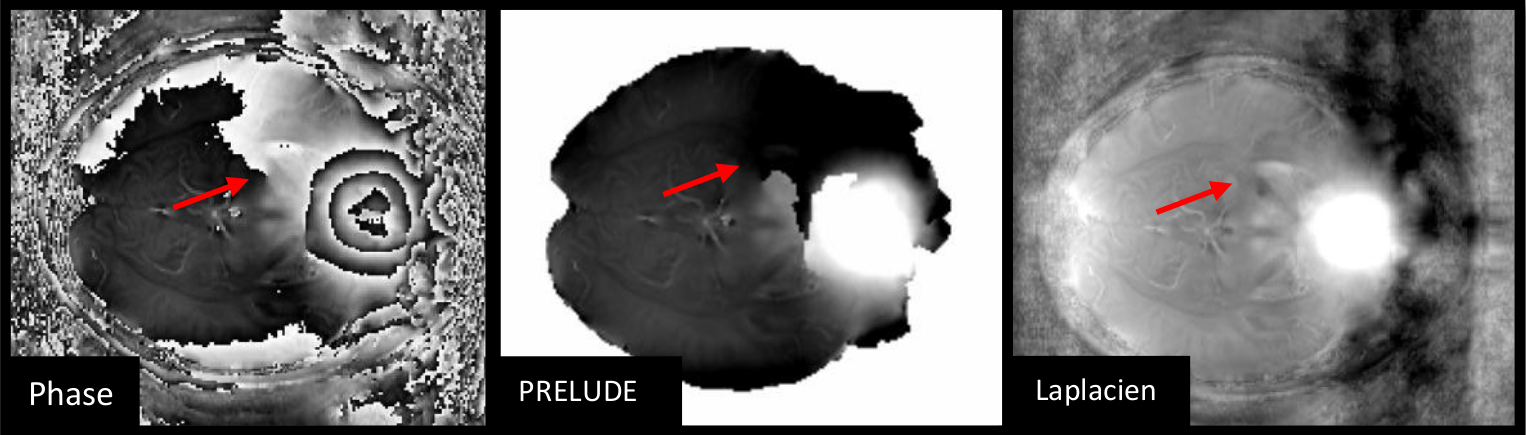
\includegraphics[width=10cm]{6_5_exemples_depliement}
\caption{Dépliement d'une phase présentant un artéfact via différents algorithmes. Le dépliement laplacien est
moins sensible à l’artéfact (flèche rouge)}
\label{fig:6_5_exemples_depliement}	
\end{figure}
%%%
%%%
\subsection{De la carte de phase à la perturbation du champ}
\label{sec:cartephasechamp}
Comme on l’a vu, la susceptibilité induit une perturbation du champ magnétique. Il est
important de noter que son effet est non local (\cite{Li2004},~\cite{Schweser2011}). Une forte susceptibilité locale aura des
retentissements à distance. Au niveau du cerveau, ce sont les interfaces air-tissu et air-crâne qui
génèrent les susceptibilités les plus importantes. Ces susceptibilités sont de l’ordre d’une dizaine de
ppm (\cite{Schenck1996}), or la valeur maximale attendue dans le tissu qui nous intéresse est d’un ppm soit un ordre
de grandeur inférieur. Le signal d’intérêt dans le cerveau va donc être pollué par des contributions
extérieures (Figure~\ref{fig:6_6_champ_interieur}). 
%%%
\begin{figure}[!t]
\centering
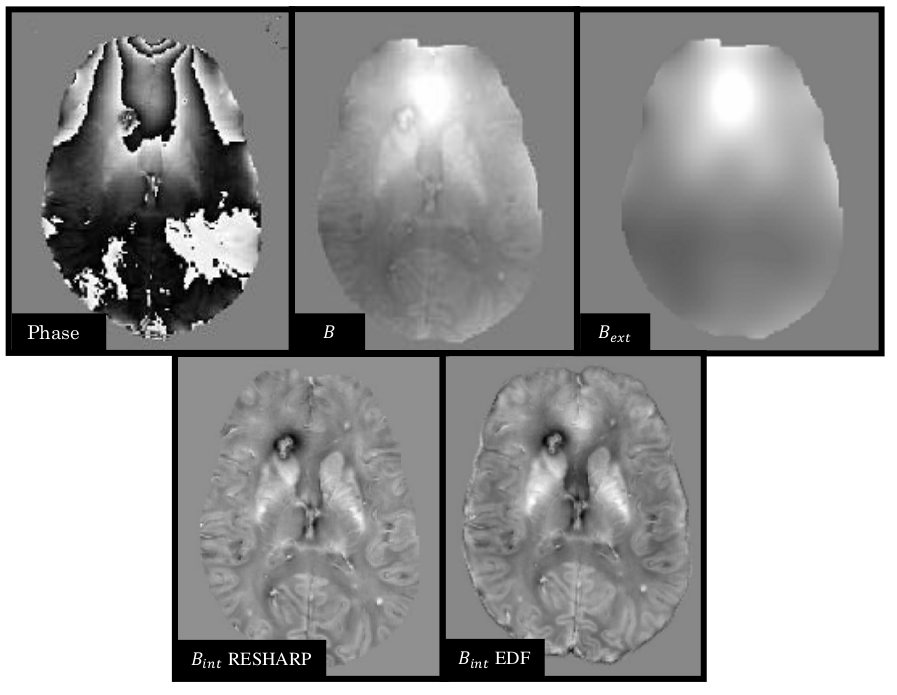
\includegraphics[width=10cm]{6_6_champ_interieur}
\caption{Cartographies de champ intérieur obtenues via RESHARP et effective dipole fitting (EDF) sur un patient
présentant des cavernomes. L’image de phase est présentée, suivi de la carte de perturbation du champ total $B$, les
contributions extérieures au champ $B_{ext}$ , le champ intérieur $B_{int}$ obtenue via l’algorithme RESHARP ou effective dipole
fitting. Les images montrent des cartographies similaires.}
\label{fig:6_6_champ_interieur}	
\end{figure}
Cependant, ces contributions extérieures varient lentement dans l’espace au
sein des régions d’intérêts. Différentes méthodes ont été proposées pour les soustraire au signal. Le
plus simple est de les filtrer sur la base d’un ajustement polynomial (\cite{Duyn2007}). D’autres utilisent la
modélisation directe pour estimer la phase via l’interface air-tissu (\cite{Neelavalli2009}). Bien que ces méthodes
paraissent adéquates pour l’élimination des contributions extérieures, leur impact détaillé sur les
variations de phases interne ne peut pas être rigoureusement précisé. Une méthode récente, nommée
« effective dipole fitting » (\cite{Liu2011b}), tente à l’inverse d’estimer la distribution de susceptibilité issue des
éléments extérieurs (interfaces etc.) qui correspond le mieux au champ dans la région d’intérêt. Elle
élimine ensuite cette contribution pour récupérer la phase intérieure (liée aux tissus). Cela est réalisé
en résolvant un problème des moindres carrés :
\begin{equation}
\chi_{out}\,=\,argmin_{\chi}\,\parallel M\bigl(B-{\cal F}^{-1}{\cal D}{\cal F}\bigr\tilde{M}\chi)\parallel_2^2,
\end{equation}
formule dans laquelle on minimise l’écart entre le champ et les effets des susceptibilités extérieures recherchées. $M$ est ici le masque du cerveau et $\tilde{M}$ son complément.\\
Une fois $\chi_{out}$ déterminé, le champ interne $B_{in}$ issu des tissus est obtenu via la formule :
\begin{equation}
B_{in}\,=\,B\,-\,{\cal F}^{-1}{\cal D}{\cal F}\,\tilde{M}\chi_{out},
\end{equation}
où $B$ est évidement obtenu à partir de la phase par l’Équation~\ref{eq:champ_phase}. $B_{in}$ représente la carte de
perturbation du champ intérieur dû aux tissus et $B$ le champ total.

L’approche est implémentée de façon itérative et, bien que très efficace, peut s’avérer couteuse en
temps.

Dans une perspective d’efficacité pour l’implémentation temps réel, Schweser et al. (\cite{Schweser2011}) ont
développé en parallèle une approche d’élimination des contributions extérieurs rapide et peu
couteuse, appelée SHARP pour Sophisticated Harmonic Artifact Reduction for Phase data.

Comme vu précédemment le champ total mesuré est la somme des perturbations du champ induite
par les tissu ($B_{in}$) et par les interfaces ($B_{ext}$ ) :
\begin{equation}
B\,=\,B_{in}\,+\,B_{ext}.
\end{equation}
Or $B_{ext}$ est entièrement dû à des sources situées à l’extérieur du volume d’intérêt (VOI), il est donc
harmonique dans tout le VOI. Cela se traduit par $\Delta B_{ext} = 0$ dans le VOI. On peut alors analytiquement
obtenir la contribution interne de $B$, $B_{int}$ en résolvant :
\begin{equation}
\Delta B\,=\,\Delta B_{in}.
\end{equation}
On peut résoudre cette équation en utilisant le théorème de valeur moyenne des fonctions
harmoniques. Ce théorème énonce qu'une fonction harmonique reste inchangée par convolution avec
un noyau parfaitement symétrique positif et normalisé (intégrale sur le noyau=1). Soit $u(\vec{r})$ la fonction
harmonique et $\rho$ le noyau, on a :
\begin{equation}
u(\vec{r})\,=\,(\rho\, \otimes\,u)\,u(\vec{r})
\end{equation}
où $\otimes$ est l'opérateur de convolution en 3D. Une série d’opérations algébrique permet alors d'éliminer
les contributions extérieures au champ comme suit :
\begin{eqnarray}
\hat{B}\,=\,B\,-\,\rho\otimes B,\\
\hat{B}\,=\,B_{in}\,+\,B_{ext}\,-\,\rho\otimes B_{in}\,-\,\rho\otimes\delta_{ext},\\
\hat{B}\,=\,B_{in}\,-\,\rho\otimes B_{in}.\label{eq:bbint}
\end{eqnarray}
$\hat{B}$ ne dépend que de $B_{in}$ et du noyau. On peut réécrire l’Équation~\ref{eq:bbint} :
\begin{equation}
\hat{B}\,=\,B_{in}\,-\,\rho\otimes B_{in}\,=\,(\delta\,-\,\rho)\,\otimes\,B_{in},
\end{equation}
où $\delta$ est un pic d’intensité 1 placé au centre du noyau $\rho$.\\
$\hat{B}$ est ensuite déconvolué à l’aide du noyau $(\delta-\rho)$ pour reconstruire $B_{in}$ :
\begin{equation}
B_{in}\,=\,(\delta\,-\,\rho)^{-1}\,\otimes\,\hat{B}.
\end{equation}
Du fait de la taille du noyau $\rho$, l'information obtenue après la convolution, $B$, est souvent corrompue
par des artefacts aux endroits où l'information n'est pas cohérente (aux limites du VOI). Il est donc
important lors de la déconvolution de ne prendre en compte que les voxels où la validité de
l'information est garantie, c'est à dire les voxels dont la convolution n'a pas été influencée par une
source de bruit. A cette fin, on utilise un algorithme de régularisation : la décomposition en valeurs
singulières tronquées (TSVD \cite{Bertero2006}). Schweser et al. (\cite{Schweser2011}) ont montré que cet algorithme permettait d'obtenir
des images contenant moins d'artefacts.

Nous avons pu confirmer sur nos données que les approches « effective dipole fitting » et
SHARP fournissent des résultats similaires (Figure~\ref{fig:6_6_champ_interieur}) (\cite{Schweser2011}).

Plus récemment une optimisation supplémentaire de la méthode SHARP a été réalisée via
l’utilisation d’une régularisation de Tikhonov à l’étape de déconvolution (RESHARP), réduisant les
erreurs dans la cartographie (\cite{Sun2014}). L’ensemble du calcul du champ intérieur et de régularisation par
TSVB est remplacé par une étape de minimisation conceptuellement similaire à celle de la méthode
« effective dipole fitting ». Le principe est de trouver la valeur de la variable $B_{in}$ qui minimise la
fonction :
\begin{equation}
argmin_{B_{int}}\,\parallel M{\cal F}^{-1}{\cal C}{\cal F}(B_{in}-B_{tot})\parallel_2^2\,+\,\lambda\parallel B_{in}\parallel_2^2,
\end{equation}
Avec $M$ le masque du cerveau érodé, ${\cal F}$ la transformée de fourrier, ${\cal C} = {\cal F}(\delta-\rho)$, $\lambda$ le paramètre de
régularisation. Dans cette formule, $argmin_{B_{in}}$ dénote les valeurs de $B_{in}$ qui minimisent la fonction ; $\parallel\,\,\parallel_2^2$ la somme des carrés ; à la différence de la minimisation effectuée dans le cadre de la méthode « effective dipole fitting », la minimisation du premier terme vise à garantir l’aspect harmonique du
champ $B_{in}-B_{tot}$ , ce qui est la base de la méthode SHARP; le second correspond à la régularisation
de Tikhonov et contrôle l’amplitude du champ $B_{in}$ ; $\lambda$ est un paramètre de régularisation dont la valeur
est fixée par la qualité de la reconstruction.

La méthode SHARP et ses dérivées impliquent par ailleurs, d’appliquer au masque du cerveau
une érosion dépendante de la taille du noyau utilisé. Cela se traduit par une perte d’information en
périphérie de l’objet. De ce fait on souhaiterait utiliser un noyau de petit diamètre, or cela engendrerait
une amplification des erreurs de phases résiduelles. Mais si le noyau est trop grand, la perte
d’information en périphérie que nous venons de mentionner sera majeure. La taille du noyau joue
donc un rôle important dans la reconstruction de la carte de perturbation du champ intérieur.
L’utilisation d’un noyau de taille variable est une solution qui permet un compromis entre la phase
extérieure résiduelle et l’intégrité de la carte reconstruite. La méthode V-SHARP (\cite{Wu2012}) utilise ainsi dans
le processus de convolution un noyau à large diamètre, qui est graduellement réduit à mesure qu’il
s’approche de la périphérie limitant les erreurs de phases tout en assurant un bon niveau d’intégrité.
%%%
%%%
\subsection{Du champ à la susceptibilité}
\label{sec:champsusc}
Rappelons que l’on doit pour finir obtenir $\chi$ en inversant :
\begin{equation}
\chi\,=\,{\cal F}^{-1}{\cal D}^{-1}{\cal F}\,B.
\end{equation}
%%%
\begin{figure}[!t]
\centering
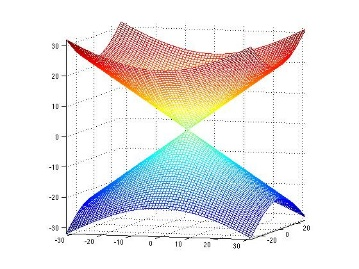
\includegraphics[width=4cm]{6_7_cone}
\caption{Illustration du cône
dans l'espace des k.}
\label{fig:6_7_cone}	
\end{figure}
Or, les fréquences spatiales auxquelles le kernel D est nul définissent une
surface conique (le long de l’angle magique, Figure~\ref{fig:6_7_cone}) dans l’espace des
$k$, qui sous échantillonne la transformée de Fourier de $\chi$ et met ainsi en
évidence le problème mal posé de l’estimation de la susceptibilité à partir
de l’image de phase. Afin d’éviter ce problème, il conviendrait de modifier
l’orientation de l’objet selon $B_0$ , ce qui a été réalisé par la méthodologie COSMOS (\cite{Liu2009b}) mais celle-ci s’avère compliquée à mettre en place et donc rarement possible.

D’autres part, la susceptiblité aura par nature une valeur relative. En effet, le kernel n’est pas
défini en son centre (division de 0 par 0), obligeant numériquement à faire un choix sur cette valeur.
Il existe plusieurs choix, la valeur 0 en ce point induit une carte de susceptibilité reconstruite disposant
d’une moyenne elle même centrée sur 0 (\cite{DeRochefort2010}), alternativement, on peut faire l’hypothèse que la carte
de champ et la distribution de susceptibilité sont différentiables selon $k_z$ ce qui amène à choisir la
valeur : -2/3 (\cite{Li2011}). Même si la seconde solution parait plus élégante, c’est la première qui est la plus
souvent employée. Le résultat est que la carte obtenue est une carte de susceptibilité relative,
déterminée à une constante près. On se concentre alors pour revenir à une valeur comparable entre
différents sujets, sur l’établissement d’une référence servant à définir notre « 0 ». Dans ce but en 2013,
Deistung et al. (\cite{Deistung2013}) ont réalisé une étude à très haut champ qui leur a permis en particulier d’idenfier
la région optimale à utiliser comme référence. Leurs résultats montrent que la matière blanche
frontale profonde est la région la plus stable et devrait en conséquence être utilisée comme référence
pour la mesure de susceptibilité.

Les difficultés liées à l’inversion du kernel ${\cal D}$ conduisent naturellement à envisager des
stratégies de régularisation qui reposent sur des connaissances supplémentaires relatives à la carte de
susceptibilité à reconstruire. En simple-T$_E$, la méthode TVSB (Total Variation Using Split Bregman) a
été développée (\cite{Bilgic2012}). Dans cette méthode on s’appuie sur l’observation suivante : les valeurs de la
susceptibilité étant liées à la nature paramagnétique de la structure sous-jacente, elles doivent varier
de façon lisse à l'intérieur des structures anatomiques d’intérêt. Dans ce cas, il est naturel de supposer
que le gradient de la susceptibilité est majoritairement faible. Pour formuler cette supposition, on cherche la distribution de $\chi$ qui correspond au mieux à la carte du champ $B_{in}$ tout en ayant un
minimum de gradient (\cite{Bilgic2012}):
\begin{equation}
\label{eq:min_gradient}
\chi_{in}\,=\,argmin_{\chi}\,\parallel B_{in}\,-\,{\cal F}^{-1}{\cal D}^{-1}{\cal F}\chi\parallel_2^2\,+\,\lambda\parallel\nabla\chi\parallel_1,
\end{equation}
Où $\parallel\nabla\chi\parallel_1$ est la norme ${\cal L}_1$ des gradients de l'image dans toutes les directions de l'espace. $\lambda$ est un
paramètre de régularisation qui permet un compromis entre les données de gradients et la continuité
spatiale de l'information. Une version alternative utilise la norme ${\cal L}_2$. Les paramètres de régularisation
sont alors déterminés sur la base de la meilleure reconstruction (\cite{Bilgic2012}). Des approches similaires telle
que l’algorithme MEDI (Morphology Enabled Dipole Inversion) (\cite{Liu2011c}) intègrent des informations de
magnitude avec des résultats proches (\cite{DeRochefort2010},~\cite{Schweser2012}). Historiquement ces approches sont utilisées sur des
séquences multi-T$_E$. 
%%%
\begin{figure}[!t]
\centering
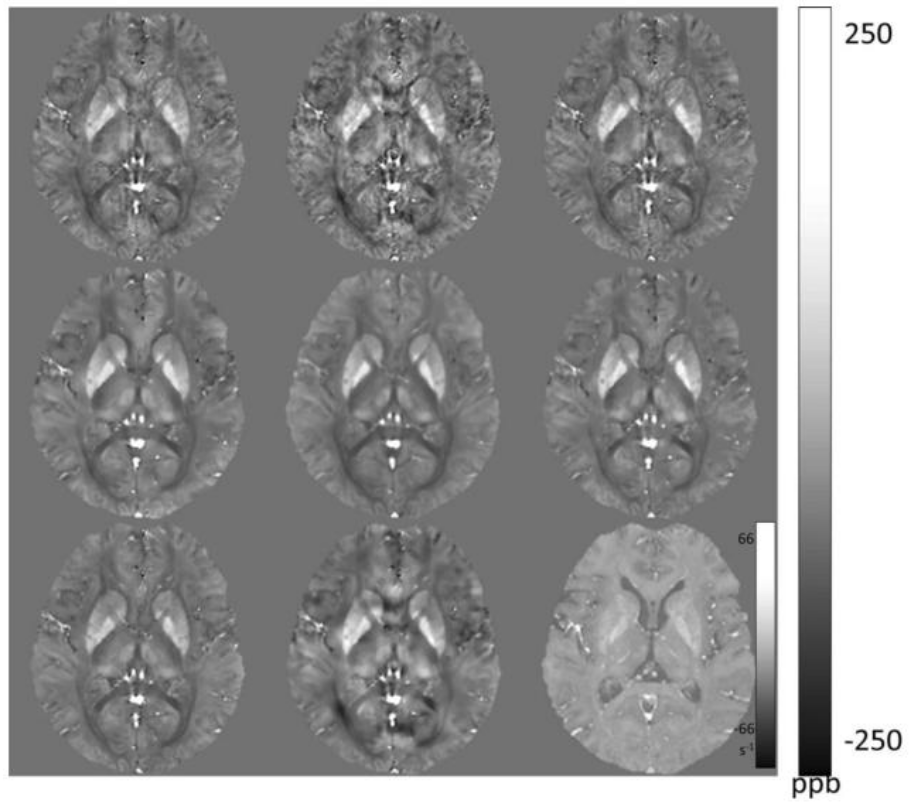
\includegraphics[width=10cm]{6_8_comparaisons}
\caption{Comparaison de différentes méthodes de reconstruction de la susceptibilité. De gauche à droite et de haut en
bas : TSVD, TKD, iSWIM, CSC, COSMOS, MEDI, HEIDI, TVSB et cartographie R2. COSMOS étant la référence. Bien que souvent
similaires, on observe la présence plus ou moins importante d’artéfacts selon la méthode utilisée. Figure issue de \cite{Wang_Liu_2014}.}
\label{fig:6_8_comparaisons}	
\end{figure}
Enfin il existe une approche simple brutale pour estimer la susceptibilité, dite TKD
(Thresholded K-space Division) (\cite{Shmueli2009}), dans laquelle on remplace dans le kernel ${\cal D}$ les valeurs inférieures
à une valeur donnée $\beta$ par $\beta^{-1}$. Cette méthode plébiscitée pour son faible coût en temps est néanmoins
sujette à de nombreux problèmes comme le choix du $\beta$ optimal, et la sous-estimation systématique de
la susceptibilité. La Figure~\ref{fig:6_8_comparaisons} présente un bilan de toutes les reconstructions (\cite{Wang_Liu_2014}).

En 2014, Bilgic et al. ont proposé une amélioration significative de la vitesse de calcul des QSM
via une optimisation de la méthode TVSB (\cite{Bilgic2013}), ouvrant la voie vers la reconstruction automatique des
cartographies de susceptibilité magnétique en ligne directement sur l’IRM en vue d’un usage clinique.
Cette méthode repose sur le fait que l’Équation~\ref{eq:min_gradient} lorsque la minimisation est formulée en norme ${\cal L}_2$
dispose d’une solution analytique :
\begin{equation}
\label{eq:bilgicanal}
\chi\,= \,({\cal F}^{-1}{\cal D}^{2}{\cal F}\,+\,\lambda\nabla^{-1}\nabla)^{-1}){\cal F}^{-1}{\cal D}{\cal F}\,B_{in}.
\end{equation}
Le gradient le long de l’axe x pouvant être représenté dans l’espace réciproque par une multiplication
avec une matrice diagonale $E_x$ :
\begin{eqnarray}
\nabla_x\,=\,{\cal F}^{-1}\,E_x\,{\cal F},\\
E_x(i,j)\,=\,1\,-\,e^{\frac{2\pi\sqrt{-1}k_x(i,j)}{N_x}}
\end{eqnarray}
Il devient possible de représenter la solution analytique sous la forme :
\begin{equation}
\chi\,=\,{\cal F}^{-1}{\cal D}[{\cal D}^2\,+\,\lambda(E_x^2+E_y^2+E_z^2)]^{-1}{\cal F}B_{in}.
\end{equation}
Le calcul de $\chi$ ne coûte plus alors que deux transformées de Fourier et la multiplication de matrices
diagonales. Cela réduit le temps de calcul d’un facteur 1000 en rapport de l’approche itérative avec
des résultats comparables (\cite{Bilgic2013}).
%%%
%%%
%%%
\section{Implémentation}
%%%
%%%
\subsection{Choix de la séquence}
Comme vu précédemment la carte de susceptibilité quantitative peut être reconstruite à partir
de séquences en écho de gradient simple ou multi-échos. Bien que la séquence multi-échos permette
de limiter la présence de certains artéfacts tout en réduisant les erreurs d’estimation de la phase, elle
augmente le temps d’acquisition. Dans le cadre de notre protocole, il est avantageux de limiter le
temps d’acquisition du fait de son intégration à un protocole clinique plus global contenant d’autres
types d’imageries. Nous avons choisi d’utiliser une séquence avec 2 temps d’échos, autorisant
l’approche décrite par Schweser et al. (\cite{Schweser2011} détaillée plus loin) permettant de détecter et retirer du
calcul les voxels aberrants par estimation de la phase initiale. Cela permet de limiter les artéfacts tout
en limitant le temps d’acquisition.

%%%
\subsection{Reconstruction de la phase}
%%%
\subsubsection{Généralités de l’acquisition d’image}
%%%
\begin{figure}[!t]
\centering
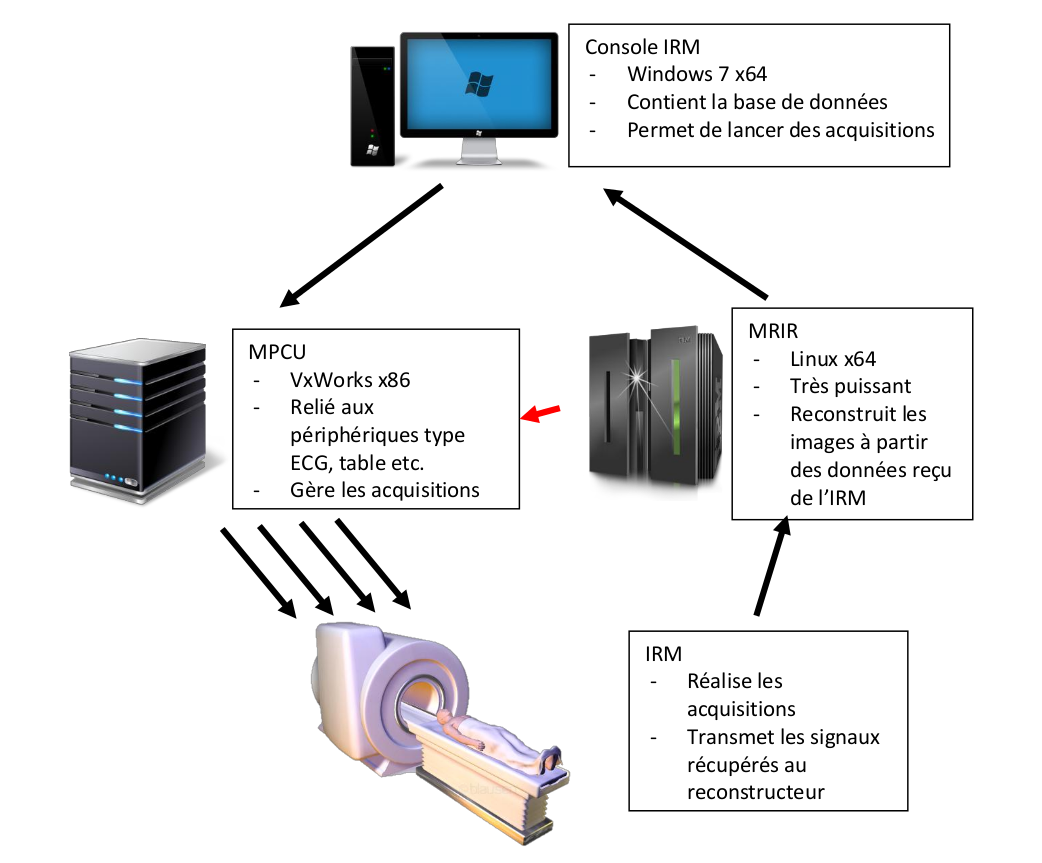
\includegraphics[width=10cm]{6_9_reconstruction}
\caption{Description du fonctionnement de la cha\^ine d'acquisition sur le système IRM.}
\label{fig:6_9_reconstruction}	
\end{figure}
Les méthodes de combinaison des différents canaux d’antennes sont adaptées à l’imagerie de
magnitude. Nous l’avons vu précédemment, des solutions existent pour recombiner correctement les
canaux et aboutir à une phase cohérente, c’est-à-dire disposant de sauts de phases cohérents (Figure~\ref{fig:6_4_ros}). Nous avons choisi d’implémenter la méthode décrite par Ros et al. (\cite{Ros2009}) via l’outil de
reconstruction ICE (Image Calculation Environment) proposé par Siemens.

Le fonctionnement d’un pipeline complet d’acquisition et de reconstruction d’image produit
par Siemens est résumé dans la figure~\ref{fig:6_9_reconstruction}.

Le système complet de reconstruction d’image est constitué de 4 éléments clés : la console
IRM, le MPCU (« Measurement and Physiological Control Unit »), l’IRM, et le reconstructeur (MRIR).

La console IRM fait l’interface entre l’IRM et l’utilisateur. Elle permet d’enregistrer les données
relatives au patient, de définir les séquences utilisées, d’ajuster les paramètres de ces séquences, et
de lancer l’acquisition. Par ailleurs, elle contient une base de données interne permettant de stocker
(temporairement) les images acquises.

La console communique avec le MPCU qui contrôle les différents périphériques de l’IRM. Il va
assurer le lancement de la séquence avec les paramètres donnés par la console.

L’IRM réalise les acquisitions, et stocke les résultats dans des fichiers bruts dit « Raw Data »
contenant des informations sur le protocole, les conditions d’acquisition (antenne etc.), les
ajustements réalisés (ajustement du bruit etc.), et surtout les données dans le plan de fourrier pour
chaque canal d’antenne. Ces données n’ont subi aucun filtrage ou traitement, elles contiennent
l’information la plus brute. En contrepartie leur taille est bien plus grande (images non recombinées
etc.) et peut atteindre une vingtaine de giga-octets avec une antenne 32 éléments. Ces fichiers sont
ainsi directement envoyés vers le reconstructeur (MRIR).

Le reconstructeur est une machine disposant à la fois d’une grande quantité de mémoire vive
et d’une forte capacité de calcul afin de gérer les grands ensembles de données des raw data, ainsi que
de capacités de parallélisation importante via l’usage des ressources des cartes graphiques Nvidia
(CUDA). Il assure en premier un rétrocontrôle vis-à-vis du MPCU (en moins de 10 ms) pour s’assurer
du bon déroulement de la séquence, puis stocke les fichiers dans un espace « tampon » pouvant
contenir une vingtaine d’acquisitions. Une fois les données copiées, la reconstruction commence.
Celle-ci va être effectuée à partir des plans de Fourier bruts, les données subissant une série de
traitements aboutissant à l’image finale au format dicom codée sur 12 bits (format dicom standard, [0
4096]). Ces images sont ensuite transférées vers la console puis archivées sur le PACS (Picture Archiving
and Communication System), tandis que les données brutes resteront, pour un temps limité sur le
reconstructeur. Elles peuvent néanmoins être récupérées manuellement par l’utilisateur via une
interface appelée TWIX.
%%%
\subsubsection{Extraction des fichiers d’intérêt des raw data}
Comme on l’a vu, c’est la méthode de Ros et al. expliquée ci-dessus qui va nous servir à
reconstruire une phase cohérente. Celle-ci requiert l’utilisation de la carte de sensibilité des canaux
d’antennes. Lors d’une séquence SWI sur machine Siemens, cette carte est obtenue via une acquisition
préalable à basse résolution (dite prescan), en utilisant l’antenne corps et l’antenne en réseau phasé. Elle n’est générée qu’une seule fois par patient. Or, ces données ne sont pas exportables au format
dicom, elles sont directement utilisées pour corriger les différences de sensibilité des différents canaux
d’antenne lorsque l’option « Prescan Normalize » est sélectionnée. Pour les récupérer il est donc
indispensable de travailler au niveau du reconstructeur afin d’intercepter les données qui nous
intéressent.

La reconstruction suit un protocole préétabli définit par la séquence utilisée. Elle se déroule
par blocs appelées « pipe ». Un pipe définit un type de traitement tel que : combinaison des canaux
d’antennes, post-traitement etc. Cette structure permet de définir des traitements à réaliser en
parallèle par le reconstructeur. La combinaison des canaux d’antenne par exemple est contenue dans
un pipe s’exécutant sur 4 threads en parallèle, chacun gérant un niveau de coupe, ce qui permet de
reconstruire le volume 3D plus rapidement. Une reconstruction complète intègre plusieurs séries de
pipe permettant de passer d’un plan de Fourier partiel à une image au format dicom.

%%%
\begin{figure}[!t]
\centering
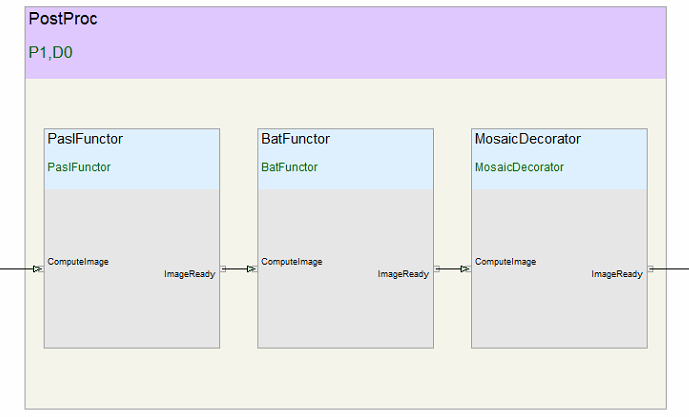
\includegraphics[width=10cm]{6_10_grase}
\caption{Exemple de pipe de type post-traitement pour une séquence ASL 3D GRASE. On distingue que ce bloc fonctionne
série (P1 = 1 thread), qu’il contient 3 functors. Le premier assure le calcul des cartes de perfusion de l’ASL (PaslFunctor), le
second détermine le temps d’arrivé du bolus (BatFunctor) et le troisième formate l’image en sortie afin d’être intégré au
format dicom (MosaicDecorator).}
\label{fig:6_10_grase}	
\end{figure}
Du point de vue de ICE, un pipe contient une série d’objets appelés « functor ». Un functor
correspond à un bloc disposant d’une fonctionnalité spécifique (calcul d’une cartographie, application
d’un facteur à l’image etc.). Cet objet est codé en C++ via la librairie ICE, il va prendre en entrée une
image (ou des lignes du plan de Fourier selon son positionnement dans la chaine de traitement), et
renvoyer en sortie une autre image. Sur la Figure~\ref{fig:6_10_grase}, on montre un exemple de pipe de post-
traitement réalisant le calcul des cartographies de perfusion et de temps d’arrivé sur des données ASL.
Comme on peut le voir, les functors se représentent sous forme de blocs reliés entre eux prenant en
entrée une ou des images, et en sortie des images traitées.

Il est possible de créer son propre functor et de l’intégrer au milieu de la reconstruction afin
de réaliser des traitements supplémentaires en ligne, ou à postériori hors ligne via un simulateur. Dans
notre cas nous souhaitons implémenter une nouvelle approche de combinaison des canaux d’antennes
qui requiert la récupération des cartes de sensibilités et des images de phase non combinées les plus
brutes possible. Nous avons choisi de sauvegarder les raw data (via l’interface dite « TWIX »), puis de
modifier le protocole de reconstruction (contenu dans les raw data) en y ajoutant des functors
permettant d’intercepter les images qui nous intéressent en vue de les traiter sous MATLAB. Cette
reconstruction est faite sur un simulateur afin de ne pas ralentir les acquisitions IRM. La Figure~\ref{fig:6_11_chaine_raw}
décrit les différentes étapes réalisés pour, à partir des raw data, aboutir à une phase cohérente.

Trois functors ont été implémentés en C++ qui ont pour objectif de sauvegarder dans un format
adapté les images de chacun des canaux (IceSaveFPArray) et de l’antenne corps (IceSaveFPBody) issue
du prescan, et les images complexes des différents canaux issue de l’acquisition SWI (IceSaveFP).

Les données issues du prescan correspondent à une couverture du crâne bien plus importante
que celle issue de l’acquisition SWI. Il est indispensable de connaitre les informations d’orientation et
de positionnement des coupes pour faire la liaison entre le prescan et l’acquisition d’intérêt. Ces
informations sont stockées dans le ICE SODA (Slice Orientation data) qui contient un ensemble
d’informations dépendantes du niveau de coupe décrivant la localisation physique des pixels d’une
image. Les functors que nous avons implémentés génèrent un ensemble de deux fichiers par image, le
premier d’extension « binHeader » contient les informations décrivant l’image : nombre de lignes,
nombre de colonnes, épaisseur de coupe, espacement des lignes, espacement des colonnes, position
sagittale, position coronale, position transverse. Le second fichier, d’extension « .dat » contient les valeurs des pixels de l’image (partie réelle et imaginaire). La combinaison de ces deux types de fichiers permettra de reconstituer le volume 3D.

%%%
\begin{figure}[!t]
\centering
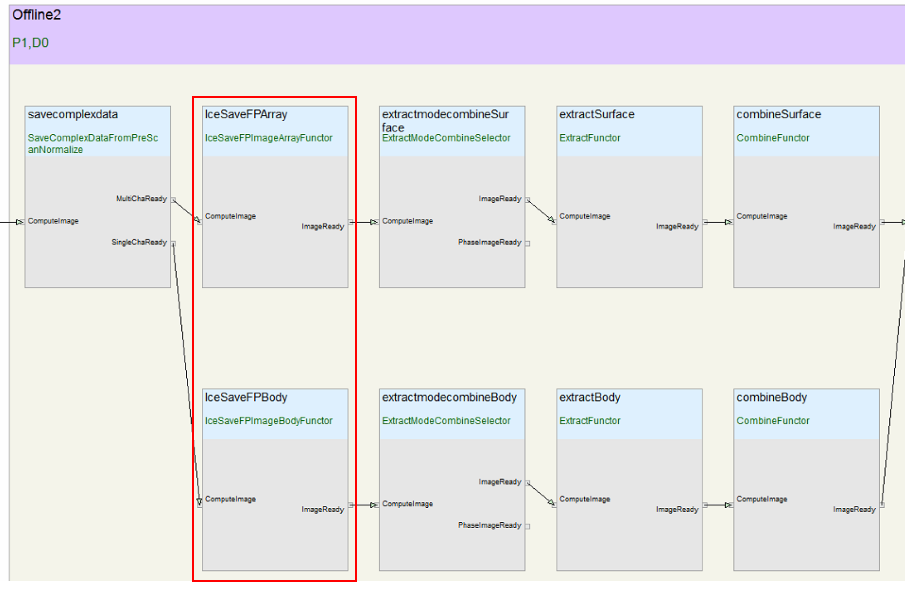
\includegraphics[width=12cm]{6_12_functors}
\caption{Positionnement des functors permettant la récupération des images issue du prescan (rectangle rouge).}
\label{fig:6_12_functors}	
\end{figure}
%%%
\begin{figure}[!t]
\centering
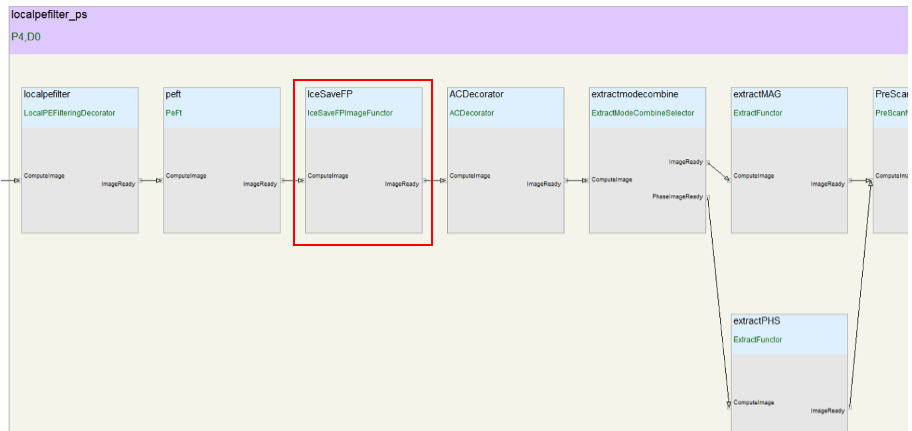
\includegraphics[width=12cm]{6_13_recuperation}
\caption{Positionnement du functors permettant la récupération des images issue de l’acquisition SWI (rectangle rouge).}
\label{fig:6_13_recuperation}	
\end{figure}
%%%

Afin de disposer d’images les plus brutes possible, ces functors ont été positionnés juste après
que les données aient subis la dernière transformée de Fourier (Figure~\ref{fig:6_12_functors} et Figure~\ref{fig:6_13_recuperation}). Il s’agit donc
de l’image la plus brute dans l’espace direct avant tout post-traitement.


%%%
\begin{figure}[!b]
\centering
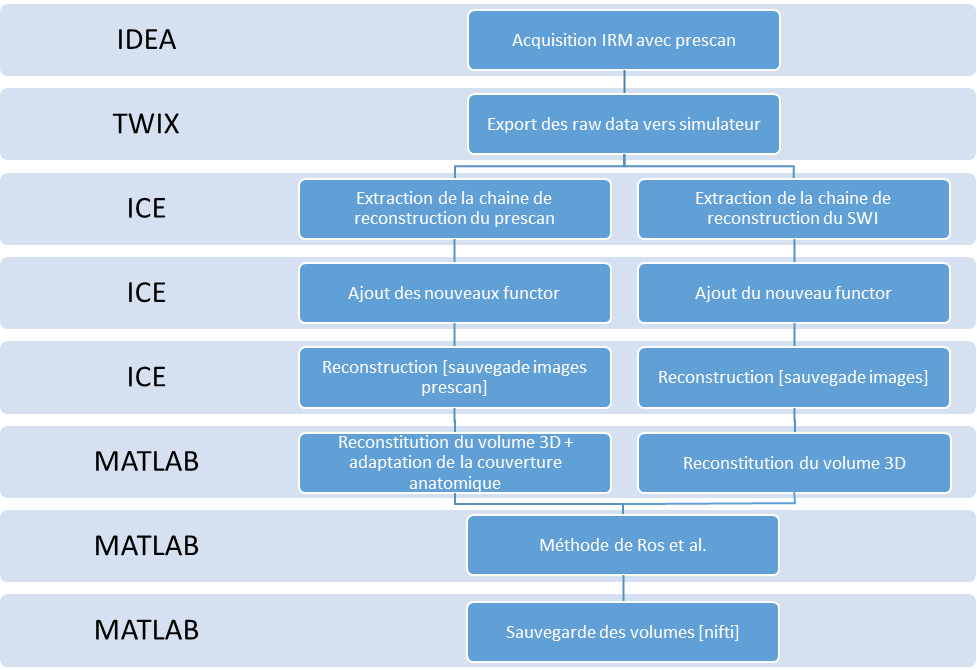
\includegraphics[width=13cm]{6_11_chaine_raw}
\caption{Principe de la chaîne de traitement permettant à partir des raw data d’aboutir à une image de phase correcte sur
un protocole SWI.}
\label{fig:6_11_chaine_raw}	
\end{figure}

\subsubsection{Sauvegarde de la phase}
Les images générées sont par la suite traitées sous MATLAB afin de réaliser la combinaison des
canaux d’antenne selon la méthode de Ros et al. (\cite{Ros2009}) comme décrit dans la partie~\ref{sec:reconstruction}. La carte de
sensibilité des différents canaux d’antenne est ainsi calculée (Figure~\ref{fig:6_14_carte_sensibilite}) et utilisée pour reconstruire
la phase et la magnitude qui seront ensuite sauvegardées au format nifti.

%%%
\begin{figure}[!b]
\centering
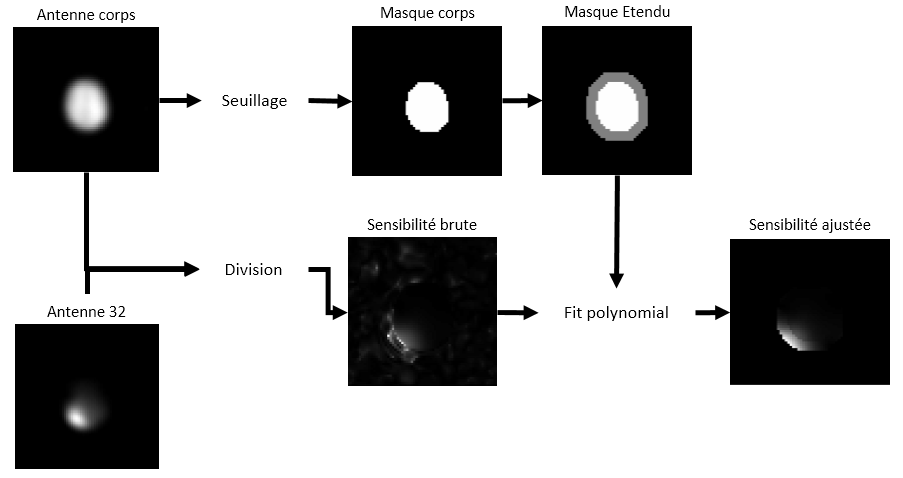
\includegraphics[width=13cm]{6_14_carte_sensibilite}
\caption{Illustration de la génération de la carte de sensibilité pour un canal d’antenne}
\label{fig:6_14_carte_sensibilite}	
\end{figure}
%%%
%%%
\subsection{Calcul de la carte de susceptibilité magnétique}
\label{sec:calcsusc}
Comme il a été montré dans les chapitres précédents (voir~\ref{sec:champsusc}), il existe de nombreux
algorithmes permettant d’aboutir à une carte de susceptibilité quantitative. Le choix d’une approche spécifique se fait sur le temps de reconstruction, la présence d’artefacts, et la difficulté
d’implémentation. Une fois la méthode choisit une optimisation doit être faite sur les paramètres de
cette méthode en terme de dépliement de la phase, de calcul de la carte de perturbation de champ
intérieur et de l’estimation de la susceptibilité (inversion).

Nous avons choisi d’utiliser l’approche de dépliement de phase laplacien (\cite{Schofield2003}) pour sa rapidité
et sa faible sensibilité aux artéfacts de phase. Les sources d’erreurs des données de la phase peuvent
inclure des artéfacts de flux non laminaires, du bruit, ou des effets de volume partiel (voir~\ref{sec:volpar}). La
séquence que nous avons choisi d’utiliser ne comporte que deux échos, on suppose pour la
reconstruction de la QSM une relation linéaire entre la phase et le temps d’écho $\frac{\phi_{T_E}}{T_E}=Cste$. Ainsi,
en principe tous les voxels de phase dont l’évolution temporelle est non linéaire peuvent, en termes
de QSM, être considérés comme incohérents. Les évolution temporelles non linaires de la phase
peuvent être déterminées à partir de deux acquisitions avec des T$_E$ différents (\cite{Schweser2011}). On utilise alors les
images de phase dépliées pour estimer la phase initiale via :
\begin{equation}
\phi^0\,=\,\phi^{T_{E_1}}\,-\,\frac{\phi^{T_{E_2}}-\phi^{T_{E_1}}}{T_{E_2}-T_{E_1}}\,T_{E_1},
\end{equation}
où $\phi^0$ est la phase initiale, $\phi^{T_{E_1}}$ la phase au temps d’écho 1, $\phi^{T_{E_2}}$ la phase au temps d’écho 2, et $T_{E_1}$
et $T_{E_2}$ les temps d’échos en ms. En imposant un aspect lissé à la distribution de la phase initiale ($\phi^0$ ) il
est possible d’identifier les voxels aberrants si ils appartiennent à des structures de haute fréquence
spatiale dans $\phi^0$ . Le critère de lissage de $\phi^0$ est justifié par l’hypothèse que cette distribution est, au
moins idéalement, dominée par la phase de la sensibilité de réception et de transmission B$_1$ (\cite{Hoult2000}). De
plus, la phase initiale ne contient aucune évolution temporelle reliée au décalage en fréquence de la
résonnance du proton. Concrètement, un ajustement d’une fonction polynomiale de degrés 4 est
effectué en 2D (tranche par tranche) puis soustrait à l’image de phase initiale $\phi^0$ . L’image résultante
est alors filtrée (filtre 3D gaussien FWHM=2.35 mm) pour réduire le bruit. Les voxels disposant d’une
valeur plus importante qu’un seuil établi empiriquement ($\pi/8$ voir \cite{Schweser2011}) sont définis comme incohérents.

La susceptibilité doit nous permettre d’accéder entre autre au compartiment veineux, que ce
soit à des fins morphologiques ou physiologiques, comme la saturation veineuse en oxygène. On a vu
que les deux principales approches d’extraction de la carte de perturbation du champ intérieur étaient
les algorithmes RESHARP et « effective dipole fitting ». Conformément à la littérature, nous avons pu
démontrer qu’elles permettent d’aboutir à un résultat très similaire (voir~\ref{sec:cartephasechamp}). L’algorithme RESHARP
propose une estimation rapide et précise de la carte de perturbation du champ intérieur, mais implique
une érosion de notre zone d’intérêt due à une violation de la propriété de la valeur moyenne lorsque le kernel de convolution chevauche la périphérie de la région d’intérêt. Or la plupart des veines qui
nous intéressent se situent en périphérie du cerveau et risquent ainsi d’être partiellement ou
totalement éliminées lors de cette étape. Bien que l’approche V-SHARP soit disponible pour limiter ce
problème, elle ne permet pas d’aboutir à une conservation suffisante des informations les plus
périphériques. L’effective dipole fitting permet d’assurer l’intégrité de la carte reconstruite, puisqu’elle
ne nécessite pas d’érosion. En contrepartie du fait de son approche complètement itérative, le temps
de calcul est plus long. Dans le cadre d’un processus de post-traitement hors ligne, la contrainte de
temps de calcul est secondaire par rapport à la qualité de la reconstruction : nous avons donc privilégié
l’effective dipole fitting.

Dans toutes ces approches, nous avons besoin d’un masque du cerveau ne contenant que le
parenchyme. La segmentation des tissus que l’on peut obtenir via des outils tels que SPM permet, par
addition des différentes cartographies de matière grise, de matière blanche et de liquide cérébro-spinal, d’obtenir une représentation assez bonne du cerveau. Cependant le temps de calcul
relativement long. FSL (FMRIB Software Library: www.fmrib.ox.ac.uk/fsl) propose une méthode dédiée
appelé BET (Brain Extraction Tool) (\cite{Smith2002}). Cette méthode utilise un modèle déformable qui évolue afin
de correspondre à la surface du cerveau par application d’un ensemble de forces locales effectives
adaptatives. L’image initiale est seuillée sur la base de son histogramme d’intensité, afin de générer
un masque binaire permettant d’évaluer le centre de gravité et le rayon de la sphère équivalente. Sur
cette base une surface en mosaïque est initialisée et par algorithme itératif, adaptée pour recouvrir
tout le cerveau. C’est un outil rapide et fiable qui permet d’extraire directement l’information qui nous
intéresse, nous l’utilisons donc comme base.

%%%
\begin{figure}[!t]
\centering
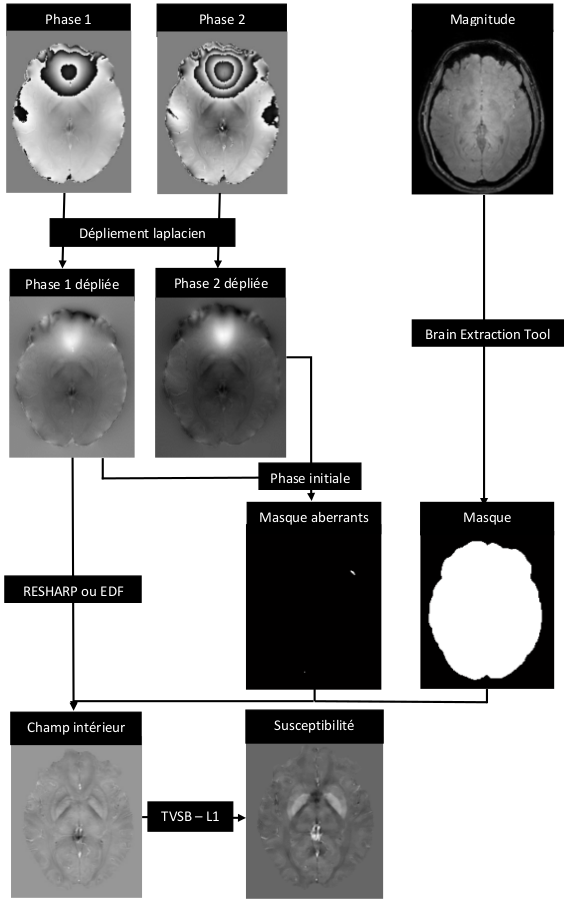
\includegraphics[width=13cm]{6_15_pipe_susceptibilite}
\caption{ Principe de la reconstruction de la susceptibilité retenue.}
\label{fig:6_15_pipe_susceptibilite}	
\end{figure}
Le passage de la carte de perturbation du champ intérieur à la susceptibilité se fait grâce à
l’optimisation la plus récente de la méthode TVSB (Total Variation Using Split Bregman) (\cite{Bilgic2014}). Qui assure
en un temps court une reconstruction de la susceptibilité en norme ${\cal L}_1$, dont nous avons pu vérifier
conformément à la littérature qu’elle était plus adaptée aux petites structures. L’approche consiste à
calculer la susceptibilité via la solution analytique de la forme ${\cal L}_2$ (Équation~\ref{eq:bilgicanal}) et de se servir de ce
résultat comme base pour calculer par itération la carte par norme ${\cal L}_1$. Le nombre total d’itérations est
ainsi réduit de façon importante, tout en conservant la qualité du résultat.

Nous obtenons ainsi une chaine complète de génération de cartographies de susceptibilité via
une séquence à deux temps d’échos. La structure des différentes opérations de post-traitement
conduisant à la carte de susceptibilité est résumée dans la Figure~\ref{fig:6_15_pipe_susceptibilite}.
%%%
%%%
%%%
\section{Validation de la mesure}
%%%
%%%
\subsection{Mise en place d’un fantôme IRM}
La QSM est une méthode relativement récente, il est donc indispensable de contrôler la qualité
et la validité des mesures réalisées. La validation est généralement faite par utilisation d’un fantôme
IRM dont l’ensemble des propriétés sont connues et contrôlées.

La susceptibilité mesure la capacité d’un matériau à s’aimanter sous l’action d’un champ
magnétique. Un fantôme de susceptibilité peut donc être réalisé via l’utilisation d’une substance
paramagnétique de composition et de concentration connues. L’équipe de Tan avec laquelle nous
avons pu échanger sur la mesure de susceptibilité dans le cadre de protocoles dédiés à la
caractérisation des cavernomes, a mis au point un fantôme de susceptibilité (\cite{tan2014}). Ce fantôme se
compose d’un sceau remplit d’eau dans lequel on plonge des tubes de type Eppendorf contenant des
concentrations variables de ferumoxytol (0 à 70 $\mu$g Fe/mL) ainsi qu’un tube de référence ne contenant
que de l’eau, l’ensemble étant maintenu par une mousse polystyrène (Figure~\ref{fig:6_16_fantome}).

%%%
\begin{figure}[!t]
\centering
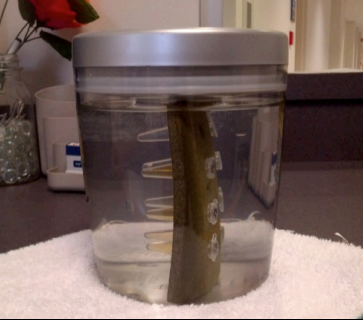
\includegraphics[width=9cm]{6_16_fantome}
\caption{Fantôme au Ferumoxytol utilisé par Tan et al. (\cite{tan2014}).}
\label{fig:6_16_fantome}	
\end{figure}
En France, le ferumoxytol n’est pas disponible, nous nous sommes donc dirigés vers une
substance de composition très similaire : le Venofer (20 mg Fe / mL). Le venofer est une solution
injectable de fer par voie intraveineuse indiquée pour le traitement de l'anémie. Pour réaliser ce
fantôme la solution de venofer a été diluée plusieurs fois afin d’obtenir une gamme allant de 0 à 60 $\mu$g
de Fe3 par mL (7 tubes). De manière à limiter les perturbations liées à la mousse qui créée de nouvelles
interfaces, nous avons choisi d’utiliser un gel d’agarose à 3 \%, transparent, moins sensible à la
formation de bulles d’air en comparaison d’autres gels. Les tubes sont remplis au maximum pour éviter
les bulles d’air puis positionnés dans une boite en plastique hermétique et maintenus après coulage
de l’agarose jusqu’à refroidissement complet. Le fantôme est ainsi transportable facilement, et
suffisamment rigide pour envisager différentes orientations dans l’IRM (Figure~\ref{fig:6_17_our_fantome}).
%%%
\begin{figure}[!t]
\centering
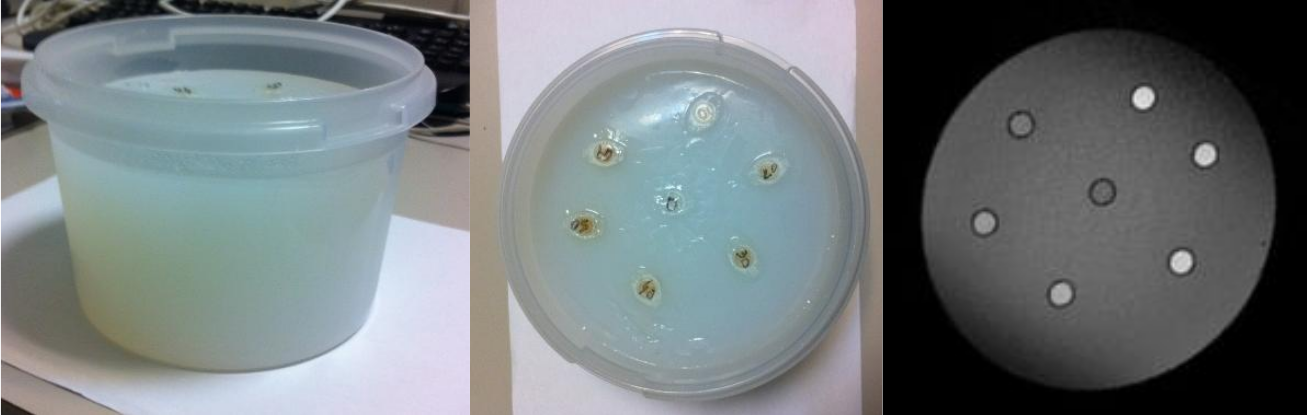
\includegraphics[width=13cm]{6_17_our_fantome}
\caption{Fantôme à base d'agarose et venofer réalisé dans cette étude. A droite, l'image en pondération
T1 est représentée avec au centre le tube contenant l'eau.}
\label{fig:6_17_our_fantome}	
\end{figure}
La susceptibilité attendue peut être estimée à partir de la concentration dans les différents
tubes. En effet, les équations de Maxwell montrent que la magnétisation d’un composé (M en A/m)
est reliée à la susceptibilité magnétique volumique ($\chi_{\nu}$ sans unité) par
\begin{equation}
\label{eq:magnetisation}
M\,=\,\chi_{\nu}\,H,
\end{equation}
où $H$ représente le champ en A/m. Or, le champ $H$ est relié au champ $B_0$ par
\begin{equation}
H\,=\,\frac{B_0}{\mu_0}\,-\,M_0,
\end{equation}
Avec le champ $B_0$ en Tesla, $\mu_0$ la perméabilité du milieu (admise à 1.256637 . 10$^{-6}$ Tm/A) et $M_0$ la
densité de magnétisation dans le milieu. En remplaçant $H$ dans l’Équation~\ref{eq:magnetisation}, on obtient :
\begin{equation}
\chi_{\nu}\,=\,\frac{M\,\mu_0}{B_0}.
\end{equation}
La magnétisation du venofer à 300°K est estimée à 6.8224 Am$^2$/kg (\cite{Gutierrez2005}), on peut donc calculer la
susceptibilité volumique du Venofer : 2.857 ppm m$^3$/kg. Cette valeur nous permettra ainsi de comparer
la concentration en fer réelle présente dans les tubes avec une concentration estimée sur la base de
la carte de susceptibilité magnétique.

Afin d’évaluer l’effet de l’orientation de l’objet dans le champ sur la reconstruction et les
différents paramètres de régularisation, nous réalisons 4 acquisitions, une en position standard à plat,
et 3 avec des inclinaisons allant jusqu’à un angle de 90°. Deux temps d’échos sont utilisés à 20 et 40
ms, la reconstruction suit ensuite le traitement décrit précédemment avec variation du $\lambda$ en norme ${\cal L}_1$
et du $\beta$ en norme ${\cal L}_2$ de l’approche TVSB.

%%%
%%%
\subsection{Validation de la méthode sur le fantôme}
Les premiers résultats mettent en évidence les problèmes liés à la régularisation avec la
présence d’artéfacts dans la direction de $B_0$ (Figure~\ref{fig:6_18_artefacts} flèches rouge). 
%%%
\begin{figure}[!t]
\centering
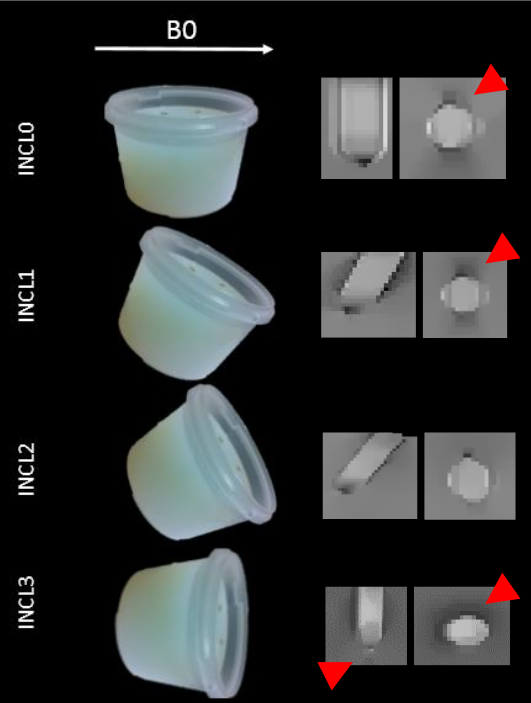
\includegraphics[width=10cm]{6_18_artefacts}
\caption{Illustration des angles d'acquisitions selon $B_0$ et susceptibilité reconstruite par norme ${\cal L}_1$ avec lambda
identique. INCL correspond à l’inclinaison. Les flèches rouges indiquent la présence d’artéfacts de reconstruction.}
\label{fig:6_18_artefacts}	
\end{figure}
Ces artéfacts vont modifier la
valeur de la susceptibiliité dans le tube. Il est donc important de choisir les paramètres de
régularisation qui limitent au mieu ces artéfacts, et d’extraire les valeurs dans des régions d’intérêt
situées à distance des interfaces.

Les effets des paramètres de régularisation sur la mesure de susceptibilité en norme ${\cal L}_1$ et ${\cal L}_2$ sont
ensuite testés. Afin d’éviter les effets de volume partiels et de limiter l’impact des artéfacts les valeurs
moyennes de susceptibilité dans les tubes sont extraites par tracage de régions d’intérêt au centre des
tubes.

Les premiers résultats sur la norme ${\cal L}_1$ mettent en évidence de bonnes corrélations entre
susceptibilité estimée et susceptibilité réelle (Figure~\ref{fig:6_19_effet_lambda}), quelle que soit la valeur du paramètre $\lambda$ la
corrélation reste très bonne. Cependant la pente de cette corrélation ne se rapproche de 1 que pour
un $\lambda$ optimal. Lorsque l’on s’en éloigne les valeurs de susceptibilité tendent à être sous estimées
(parfois même fortement). En observant l’évolution du coefficient de corrélation en fonction du $\lambda$ pour
la norme ${\cal L}_1$ (Figure~\ref{fig:6_19_effet_lambda}), on peut mettre en évidence la valeur optimale (Figure~\ref{fig:6_19_effet_lambda} ligne en pointillé
rouge). 

Le même type de résultat est observé avec la norme ${\cal L}_2$ (résultats non présentées ici).
Cependant, pour cette norme même pour le $\beta$ optimal, il existe une sous estimation de la susceptibilité
(pente distante de 1). La comparaison des valeurs obtenues par norme ${\cal L}_1$ et ${\cal L}_2$ après sélection du
paramètre adapté met en évidence une sous-estimation en norme ${\cal L}_2$ des concentrations estimées en
rapport des vrais valeurs (p=0.015, Wilcoxon unilatéral pairé), tandis qu’en norme ${\cal L}_1$ les valeurs ne
sont pas significativement différentes de la concentration réelle (p>0.05, Wilcoxon unilatéral pairé). La
norme ${\cal L}_1$ semble donc à privilégier pour l’extraction de valeurs quantitatives, même si, en terme de
corrélation, la norme ${\cal L}_2$ reste correcte (p<<0.01, rho=0.99, corrélation de Pearson). Cet essai permet
d’apporter une validation de la mesure de susceptibilité sur l’IRM à notre disposition dans des
conditions standards d’acquisition.

%%%
\begin{figure}[!t]
\centering
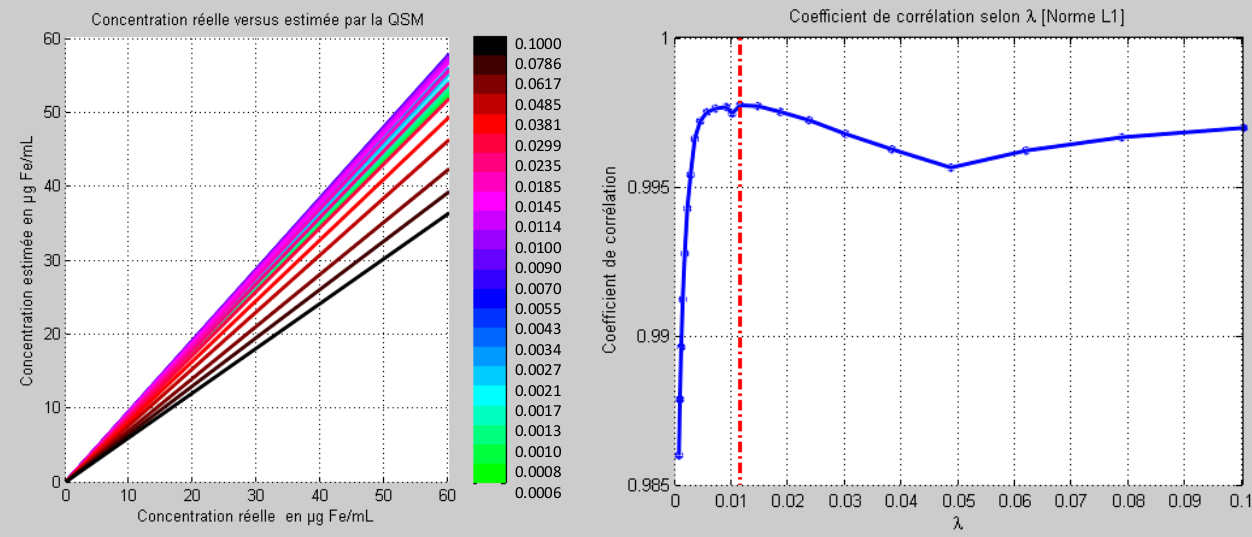
\includegraphics[width=13cm]{6_19_effet_lambda}
\caption{Effet du paramètre lambda dans la reconstruction de la carte de susceptibilité magnétique. A gauche la
comparaison entre concentration estimée et concentration réelle en fonction du paramètre lambda choisi. Les courbes sont
ajustées linéairement. A droite, le coefficient de corrélation (Pearson) est représenté en fonction du lambda. Le coefficient le
plus important est indiqué par le trait rouge (0.0114).}
\label{fig:6_19_effet_lambda}	
\end{figure}


%%%
\begin{figure}[!b]
\centering
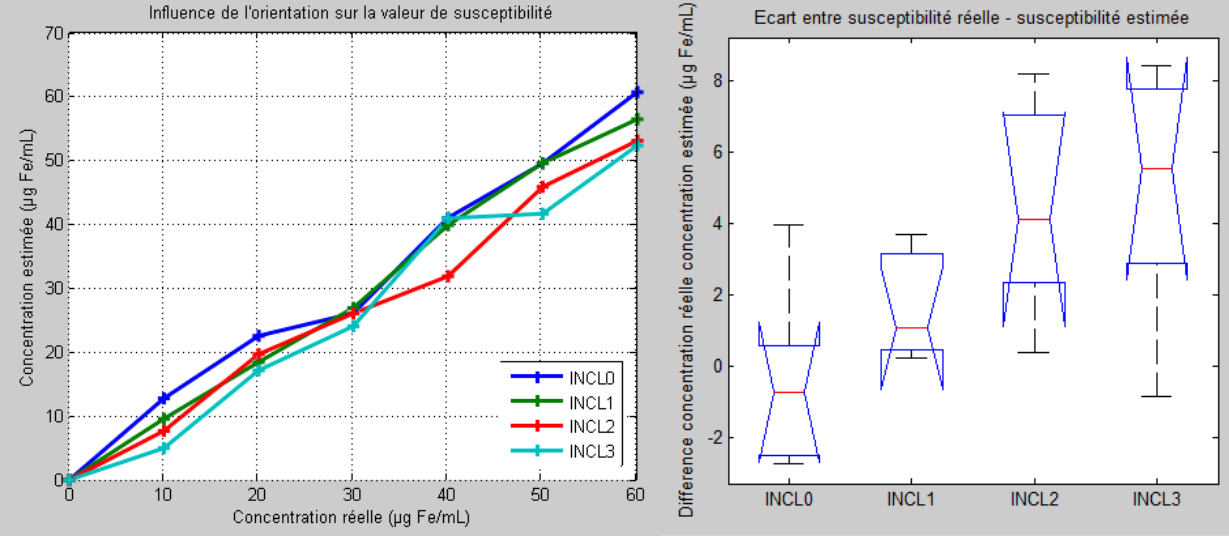
\includegraphics[width=13cm]{6_20_orientation}
\caption{Influence de l'orientation sur la mesure de susceptibilité. A gauche, les courbes de concentration réelle versus
estimées pour les différentes inclinaisons. A droite des boites à moustaches illustrant l'écart entre la valeur réelle et la valeur
estimée. INCL0 à 3 représente les différentes orientations, 0 étant la position de référence.}
\label{fig:6_20_orientation}	
\end{figure}
L’impact de l’orientation de l’objet dans le champ doit aussi être testé. En effet, nous l’avons
vu sur la Figure~\ref{fig:6_18_artefacts}, l’orientation peut être la cause de la présence d’artéfacts de reconstruction sur la
cartographie finale. La Figure~\ref{fig:6_20_orientation} illustre l’impact de l’orientation sur la mesure de susceptibilité.
Comme on peut le voir, l’orientation par rapport au champ modifie significativement la susceptibilité
(p<0.05, Kruskal Wallis). Il existe une correlation entre l’inclinaison et la différence entre concentration
réelle concentration estimée (p<0.05, rho=0.97, correlation de Pearson). Lorsque le tube est parallèle
au champ (INCL3), l’erreur de reconstruction entraîne une diminution sensible de la valeur mesurée.

La prise en compte de ce type de résultat est importante lors de l’utilisation de la méthodologie
QSM, et reste trop peu généralisée. Il est particulièrement important de connaitre l’orientation des
structures dont on souhaite estimer la susceptibilité, afin de maitriser la fiabilité de la mesure. Par
exemple, dans le cadre qui nous intéresse de la susceptibilité des veines, l’orientation de certaines
veines vis-à-vis du champ magnétique pourra modifier leur susceptibilité sur la carte reconstruite. Lors
de l’exploitation des résultats il est important de se rappeler que toutes les valeurs de susceptibilité le
long des veines ne sont pas de la même fiabilité.
%%%
%%%
\subsection{Retour au cerveau : multi-temps d’échos ou simple écho ?}
La réalisation du fantôme ayant permis de valider la mesure de susceptibilité dans un cadre
contrôlé, nous pouvons maintenant tester cette reconstruction sur des données réelles d’imagerie.
Comme nous l’avons mentionné, l’acquisition de plusieurs temps d’échos (typiquement 8) permet de
limiter la présence d’un certain nombre d’artéfacts. Nous avons donc voulu nous assurer que
l’utilisation d’une approche limitée à un temps d’écho permettait d’obtenir des résultats similaires
dans le cadre de notre chaine de traitement.

Une acquisition à 8 temps d’échos (6 à 63 ms linéairement répartis) avec un T$_R$ de 70 ms a été
réalisée pour tester la reconstruction multi-TE associée à l’approche couramment utilisée dans ce cas :
l’algorithme dédié « MEDI » (Morphology Enabled Dipole Inversion) (\cite{Liu2011b}). Ce type d’acquisition génère
des données de très grosse taille. Du fait de notre mode de reconstruction et du matériel disponible,
nous sommes limités à une taille maximale de 8 Go par raw data. Il a donc été nécessaire d’utiliser une
imagerie parallèle GRAPPA correspondant à un sous échantillonnage d’un facteur 3 de l’espace
réciproque.

Pour comparer les différents modes de reconstruction, nous avons testé plusieurs approches :
\begin{itemize}
	\item En multi-TE : Les valeurs de la phase le long des temps d’échos sont ajustées pour en extraire
	la pente qui sert de base à la reconstruction
	\begin{itemize}
		\item Norme L1 : via l’algorithme TVSB.
		\item Norme L2 par utilisation de la magnitude : via l’algorithme MEDI (\cite{Liu2011b})
	\end{itemize}
	\item Simple temps d’écho : On comparera une acquisition simple-TE pour deux d’échos données
	(court et long)
	\begin{itemize}
		\item Norme L1 : via l’algorithme TVSB
		\begin{itemize}
			\item Sur la base d’un temps d’écho long
			\item Sur la base d’un temps d’écho court
		\end{itemize}
	\item Norme L2 : via l’algorithme TVSB
	\end{itemize}
\end{itemize}
Dans tous les cas, le calcul de la carte de perturbation du champ intérieur est réalisé via la
méthode RESHARP.

%%%
\begin{figure}[!t]
\centering
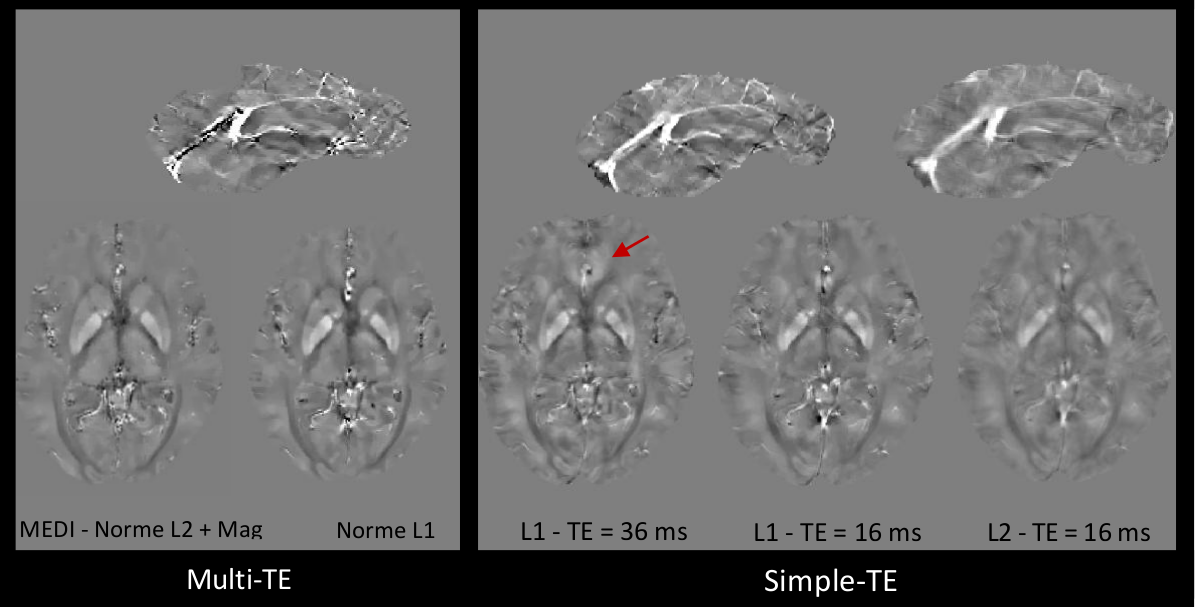
\includegraphics[width=13cm]{6_21_multi_simple_te}
\caption{Comparaison multi-T$_E$ versus Simple-T$_E$. La flèche rouge indique la présence d’artéfacts liés à des erreurs
lors de l’estimation de la carte de perturbation du champ intérieur lorsque les sauts de phases sont importants.
L’échelle utilisée est la même pour toutes les images.}
\label{fig:6_21_multi_simple_te}	
\end{figure}
\begin{figure}[!b]
\centering
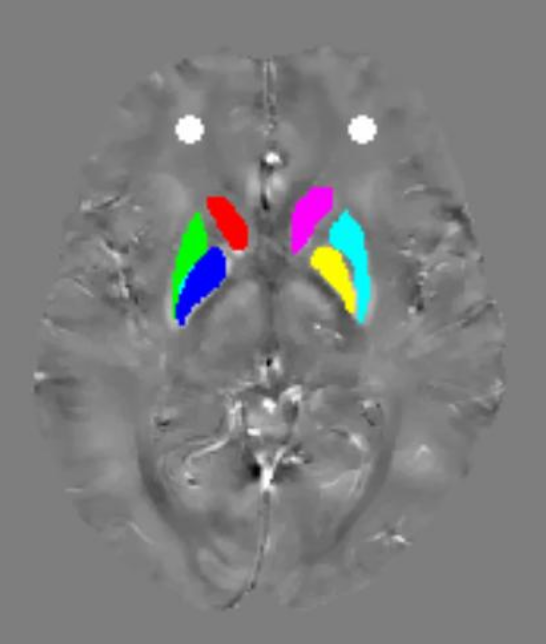
\includegraphics[width=7cm]{6_21b_ill_roi}
\caption{Illustration de quelques ROI sélectionnées. Ici matière blanche, putamen, pallidum et noyau caudé
superposées sur la norme ${\cal L}_1$, $T_E$= 16 ms.}
\label{fig:6_21b_ill_roi}	
\end{figure}
Nous pouvons donc dans ce protocole évaluer qualitativement le mode multi-T$_E$ versus simple-
T$_E$, mais aussi l’impact du temps d’écho et de la norme sur l’estimation de la susceptibilité et la visibilité
des différentes structures en simple-T$_E$. La Figure~\ref{fig:6_21_multi_simple_te} illustre la reconstruction de la carte de
susceptibilité dans différentes conditions. Comme expliqué précédemment un temps d’écho plus long
permet d’aboutir à un meilleur contraste. Cependant cela implique des déphasages beaucoup plus
importants et donc des difficultés supplémentaires lors du dépliement de la phase et lors de
l’extraction de la carte de perturbation du champ intérieur. Il en résulte des artéfacts (Figure~\ref{fig:6_21_multi_simple_te} flèche
rouge) sur la carte reconstruite, très peu visibles avec un temps d’écho plus court. L’approche multi-
T$_E$ ne présente pas ces artéfacts. Concernant les structures telles que les veines, il semble que
l’approche simple-T$_E$ en norme ${\cal L}_1$ permette de les mettre en évidence plus clairement. La norme ${\cal L}_2$
semble en revanche « lisser » la cartographie finale, limitant la visibilité de ces structures. Enfin, on
détecte visuellement une susceptibilité moyenne plus faible en norme ${\cal L}_2$ (comme cela a été montré
via le fantôme) en comparaison de la norme ${\cal L}_1$.

Pour comparer enfin les informations quantitatives, nous avons choisi de définir différentes
régions d’intérêt au niveau des noyaux gris : pallidum, putamen, noyaux caudés, noyaux dentelés dans
les deux hémisphères, ainsi que deux sphères (5 mm de rayon) dans la matière blanche frontale (Figure~\ref{fig:6_21b_ill_roi}) pour servir de référence à la valeur de susceptibilité (\cite{Schweser2011}). Nous avons donc au total 10 ROI plus
une de référence.

Cette analyse a été réalisée sur la base d’un même jeu de données (une même acquisition à 8
temps d’échos) et pour une même information extraite, la susceptibilité. Il est donc compliqué
d’utiliser des tests statistiques standards pour évaluer directement les différences quantitatives entre les modes de reconstruction. Pour apprécier la concordance des mesures, des graphiques de Bland-
Altman ont été réalisés. La susceptibilité rapportée est recentrée sur la valeur moyenne de la substance
blanche frontale.

Pour clarifier les résultats nous ne nous intéresserons qu’à la norme ${\cal L}_1$ en simple T$_E$ (T$_E$ court)
et la norme ${\cal L}_2$ via l’algorithme MEDI en multi-T$_E$ car ces deux approches sont les plus citées dans la
littérature récente (\cite{Wang_Liu_2014}).
\begin {table}
\caption{Mesures de la susceptibilité pour différents noyaux gris selon différents modes de reconstruction. Les valeurs
sont exprimées en ppm, et la matière blanche sert de référence.} 
\label{tab:susceptbilite} 
\centering
\begin{tabularx}{\linewidth}{X c c c c}
\hline
 & \multicolumn{2}{c}{{\bf Simple T$_E$ (T$_E$ = 16 ms) }} & \multicolumn{2}{c}{{\bf Multi-T$_E$}} \\
\hline
 & ${\cal L}_1$ & ${\cal L}_2$ & ${\cal L}_2$ MEDI & $ {\cal L}_1$\\
\hline
{\bf Noyaux caudés gauche } & 0,0189  &  0,0229 &  0,0255 & 0,0213 \\
\hline
{\bf Pallidum gauche } & 0,0730  & 0,0688  & 0,0732 & 0,0680 \\
\hline
{\bf Putamen gauche } &  0,0095 &  0,0139 & 0,0188  & 0,0133 \\
\hline
{\bf Noyaux dentelés gauche} & 0,0230  &  0,0199 & 0,0308 &0,0223 \\ 
\hline
{\bf Noyaux rouges gauche } & 0,0426   & 0,0406  &  0,0395 & 0,0400\\ 
\hline
{\bf Noyaux caudés droit } & 0,0255 & 0,0251 &  0,0256 &  0,0217\\
\hline
{\bf Pallidum droit } &0,0765   &  0,0688 &0,0681  & 0,0616 \\
\hline
{\bf Putamen droit } &  0,0220 &  0,0235 & 0,0174 &0,0106\\ 
\hline
{\bf Noyaux dentelés droit} & 0,0258  & 0,0198  & 0,0177& 0,0164 \\ 
\hline
{\bf Noyaux rouges droit } & 0,0335  &  0,0371 & 0,0569  &0,0414 \\ 
\hline
{\bf Matière blanche} &  0&  0&  0& 0\\ 
\hline
\end{tabularx}

\end{table}
Les valeurs observées sont illustrées dans le Tableau~\ref{tab:susceptbilite} pour les différentes conditions et
régions. Ces résultats sont résumés dans le graphique de Bland-Altman (Figure~\ref{fig:6_22_bland}). Comme on peut le
voir sur le graphique de droite, la différence entre les deux mesures est bien centrée sur 0 avec une
variabilité très faible entre les mesures. De plus la concordance entre les deux mesures semble bonne
avec une courbe (à gauche) qui se rapproche fortement de la courbe de référence à 45°. Nous avons
par ailleurs calculé le coefficient de concordance de Lin (\cite{Lin1989}) afin d’évaluer plus clairement la fiabilité
inter-méthode. L’analyse montre une bonne concordance des deux méthodes (coefficient de
corrélation de concordance = 0.92 ; Pearson $\rho$ = 0.92 ; Facteur de correction du biais Cb = 0.99) au vu
des seuils rapportés dans la littérature (\cite{Mcbride2005}). Il semble donc que les deux méthodes fournissent dans
notre configuration des résultats similaires.

%%%
\begin{figure}[!t]
\centering
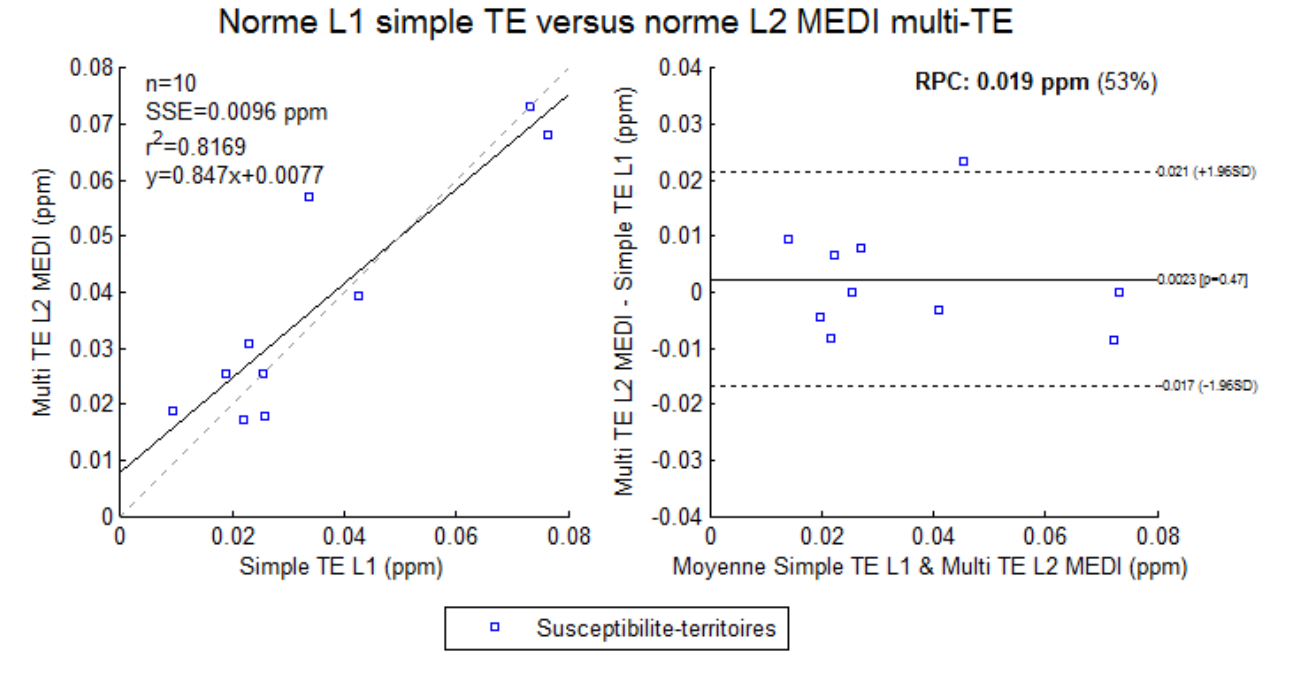
\includegraphics[width=13cm]{6_22_bland}
\caption{Analyse de Bland-Altman pour comparer les méthodes de reconstruction Multi-T$_E$ norme ${\cal L}_2$ MEDI et simple T$_E$
norme ${\cal L}_1$. A gauche est représenté la corrélation des deux méthodes, avec en pointillés la courbe de référence à 45°, à droite
la différence entre les deux mesures en fonction de la moyenne des deux.}
\label{fig:6_22_bland}	
\end{figure}
Nous pouvons donc utiliser des séquences de type simple-TE offrant l’avantage de réduire le
temps d’acquisition tout en conservant une qualité de résultat suffisante pour extraire des résultats
fiables.
%%%
%%%
\subsection{Création d’une toolbox SPM}
Les différentes méthodes de validation nous ont montré la fiabilité de notre chaine de
traitement et la conformité des résultats avec les approches courantes de la littérature. Afin d’unifier
et surtout faciliter l’accès à la cartographie de susceptibilité magnétique, nous avons intégré le calcul
de la QSM à SPM via la création d’une boite à outils (toolbox) nommée « ELLIS ». Cet outil permet de
réaliser le traitement depuis l’extraction du cerveau, en passant par le dépliement de la phase et le
calcul du champ intérieur pour enfin aboutir à la susceptibilité (Figure~\ref{fig:6_15_pipe_susceptibilite}).

La création d’une boite à outils intégrée à SPM nécessite 4 fichiers principaux assurant la
définition de l’environnement, la définition des paramètres rentrés par l’utilisateur, le calcul et enfin
l’affichage de l’aide.

Le premier fichier « spm\_ELLIS.m » sert d’entrée et définit le nom de la boite à outils, les
répertoires contenant les fonctions d’intérêt, le chemin vers le fichier d’aide. Le second « ELLIS.man »
représente l’aide de la boite à outils, affichée au démarrage de l’outil. Le troisième «tbx\_cfg\_ELLIS.m »
contient la définition des différents champs qui devront être renseignés ou sélectionnés par
l’utilisateur, pour être ensuite donnés en argument à la fonction de calcul de la susceptibilité. La
création d’un champ est réalisée comme suit :

{\tt
\begin{tabbing}
\hspace{1cm}\=\hspace{1cm}\\
\> qsm\_phaseTE2 = cfg\_files; \textcolor{green}{\% type de champ}\\
\> qsm\_phaseTE2.tag = \textcolor{red}{'qsm\_phaseTE2'}; \textcolor{green}{\% identifiant du champ}\\
\> qsm\_phaseTE2.name = \textcolor{red}{'First phase image (TE2)'}; \textcolor{green}{\% label affiché àl'utilisateur}\\
\> qsm\_phaseTE2.help = \{[...\\
\> \textcolor{red}{'Image should range from -pi to +pi, if no rescale is done.'}...\\
\> \textcolor{red}{'Used to generate QSM and estimate initial phase.'}...\\
\> \textcolor{red}{'cf RESHARP.'}]\}; \textcolor{green}{\% Aide}\\
\> qsm\_phaseTE2.filter = \textcolor{red}{'image'}; \textcolor{green}{\% type de données rentrées}\\
\> qsm\_phaseTE2.ufilter = \textcolor{red}{'\^.*'}; \textcolor{green}{\% filtre à utiliser}\\
\> qsm\_phaseTE2.num = [1 1]; \textcolor{green}{\% nombre de données à rentrer}\vspace{0.5cm}\\
\end{tabbing}
}
Par ailleurs on y définit la fonction qui va recevoir en argument les données de ces champs.
Cette fonction appelée « ps\_qsmmapping\_run.m » dans notre cas réalise l’ensemble du traitement et
se charge d’afficher les images intermédiaires dans la fenêtre de visualisation de SPM. La fonction
reçoit en entrée une variable « job » regroupant l’ensemble des champs présents dans l’interface et
définis dans le fichier « tbx\_cfg\_ELLIS.m ». Les données peuvent donc être récupérées facilement :
 
{\tt
\begin{tabbing}
\hspace{1cm}\=\hspace{1cm}\\
\> \textcolor{blue}{function} varargout = ps\_qsmmapping\_run( job,arg )\\
\> \textcolor{green}{\% function calculant la carte de susceptibilité}\\
\> \textcolor{green}{\% la variable job contient les champs renseignés}\\
\> \textcolor{green}{\% par l’utilisateur}\\
\> \textcolor{green}{\%\% recuperation des arguments}\\
\> phase1\_path = job.qsm\_phase.qsm\_phaseTE1{1};\\
\> phase2\_path = job.qsm\_phase.qsm\_phaseTE2{1};\\
\> mag\_path = job.data\_qsm\_mag{1};\\
\> TE1 = job.qsm\_params.qsm\_TE1;\\
\> TE2 = job.qsm\_params.qsm\_TE2;\\
\> res = job.qsm\_params.qsm\_reso;\\
\> B0 = job.qsm\_params.qsm\_B0;\\
\> doSegment = job.qsm\_params.qsm\_doSegment;\\
\> sharp\_radius = job.qsm\_calcp.qsm\_sharpKernel;\\
\> Lnorm = job.qsm\_calcp.qsm\_norm;\\
\> useMag = job.qsm\_calcp.qsm\_magweight;\\
\> useDefLambda = job.qsm\_calcp.qsm\_useDefLambda;\\
\end{tabbing}
}
La création de ces différents fichiers permet de faire apparaitre la boite à outils dans SPM.
%%%
\begin{figure}[!t]
\centering
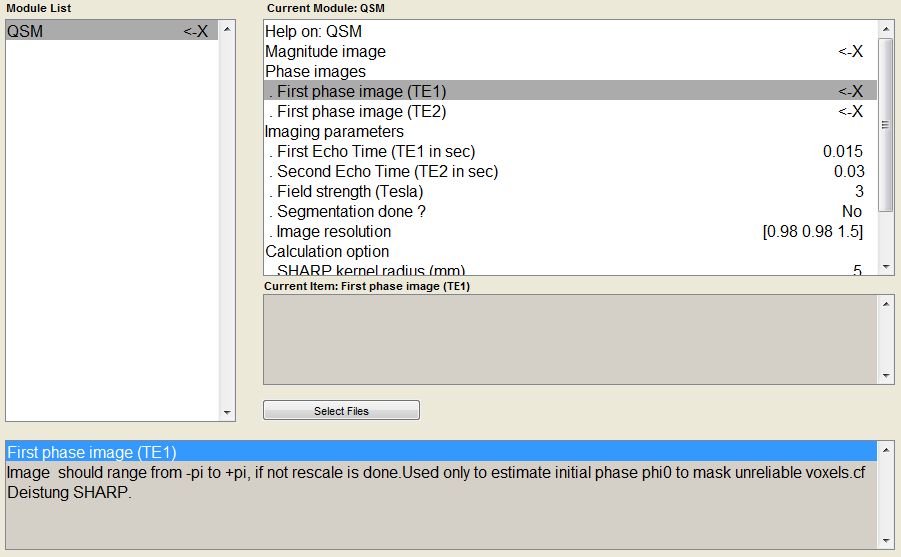
\includegraphics[width=13cm]{6_23_toolbox}
\caption{Toolbox QSM pour SPM (interface Batch)}
\label{fig:6_23_toolbox}	
\end{figure}
Dans l’interface créée (Figure~\ref{fig:6_23_toolbox}), l’utilisateur renseigne les chemins vers deux images de phases et
une image de magnitude, ainsi que les paramètres clefs de l’acquisition (champ, temps d’échos,
résolution). Il lui est ensuite proposé de sélectionner la taille du kernel si l’algorithme RESHARP est
utilisé, et le type de calcul de la susceptibilité : norme ${\cal L}_1$ ou ${\cal L}_2$ avec détection automatique des
paramètres optimaux (\cite{Bilgic2014}) ou non, et pondération par la magnitude ou non. Les images de phase brutes
et dépliées, ainsi que le champ intérieur et la carte finale de susceptibilité, sont affichées au cours du
traitement. Son intégration à SPM permet de l’associer à d’autres types de traitements dans des
« batchs » plus généraux. En effet, le système batch de SPM permet de mettre en série différents
traitements très simplement, il devient par exemple aisé de calculer la QSM puis de normaliser la
cartographie en rajoutant un bloc « normalize » qui récupère l’image du précédent bloc pour s’en
servir comme base.

Cet outil a permis, après validation via le fantôme, de réaliser des études annexes. Une
première associe tenseur de diffusion et susceptibilité magnétique dans le cadre de la caractérisation
des différentes formes de pathologies parkinsoniennes (\cite{Dunet2015}). Une seconde étudie les différents types
de cavernomes (familiaux et sporadiques) à travers leur évolution en susceptibilité (\cite{Balasse2015}). Et une
dernière met en évidence des effets jusqu’alors non décrit dans littérature dans le cadre des
leucoencéphalopathie multifocale progressive (\cite{Carra2015}).

%%%
\begin{figure}[!t]
\centering
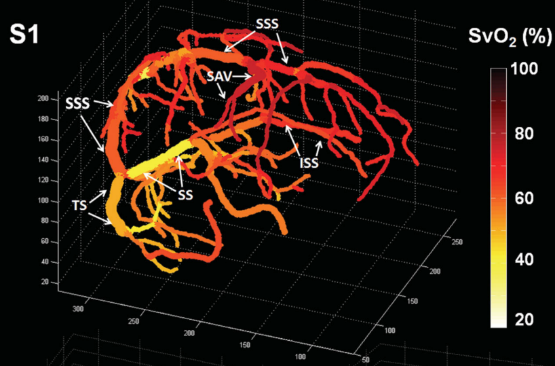
\includegraphics[width=9cm]{6_24_ex1}
\caption{Cartographie de saturation en oxygène dans les veines. Illustration issue de \cite{Fan2014}.}
\label{fig:6_24_ex1}	
\end{figure}
%%%
%%%
\subsection{Applications}
Les cartographies de susceptibilité permettent de segmenter facilement les veines par simple
seuillage sur la base de la valeur en ppm. Du fait de la résolution plus fine que celle de l’imagerie en
contraste de phase, cette imagerie peut permettre d’accéder à des vaisseaux plus petits. La
visualisation des veines est rendue possible par le fait que le sang qu’elles contiennent est désoxygéné.
Le sang artériel est en effet riche en oxygène, et contient donc avec une concentration importante
d’oxyhémoglobine. La combinaison du Fer (Fe$^{2+}$) et de l’oxygène donne un composé diamagnétique.
Une fois désoxygénée, l’hémoglobine (devenue déoxyhémoglobine), devient paramagnétique et
apparait donc hyperintense en QSM (\cite{Wang_Liu_2014}). Le décalage de susceptibilité entre le sang veineux et l’eau
($\Delta_{\chi vein-water}$ ) est donc dominé par la concentration oxygène-dépendante de la déoxyhémoglobine
paramagnétique dans le sang. Cette différence de susceptibilité est reliée à la saturation en oxygène
(SvO$_2$) dans le vaisseau selon la formule (\cite{Weisskoff1992}) :
\begin{equation}
\Delta_{\chi_{vein-water}}\,=\,(1-SvO_2)\,\Delta_{\chi do}\,Hct\,+\,\Delta_{\chi oxy-water},
\end{equation}
Avec $Hct$ le pourcentage d’érythrocytes dans le sang, $\Delta_{\chi do}$ le décalage de susceptibilité par unité
d’hématocrite entre le sang complètement oxygéné et les érythrocytes désoxygénés, et $\Delta_{\chi oxy-water}$ le
décalage de susceptibilité entre les cellules sanguines oxygénées et l’eau.\\
Les valeurs de $\Delta_{\chi do}$ , $\Delta_{\chi oxy-water}$, et $Hct$ peuvent être récupérées dans la littérature
(\cite{Spees2001},~\cite{Fan2014},~\cite{Weisskoff1992}) avec respectivement 0.27 ppm (cgs), -0.03 ppm et 40 \%. Il devient alors aisé d’extraire
la saturation en oxygène dans les veines (Figure~\ref{fig:6_24_ex1}, Figure~\ref{fig:6_25_ex2}). Des extensions de ces approches ont
été développées afin d’appréhender la consommation en oxygène dans les tissus (CMRO2) par
utilisation conjointe de l’ASL et de la QSM (\cite{Zhang2014}).
%%%
\begin{figure}[!t]
\centering
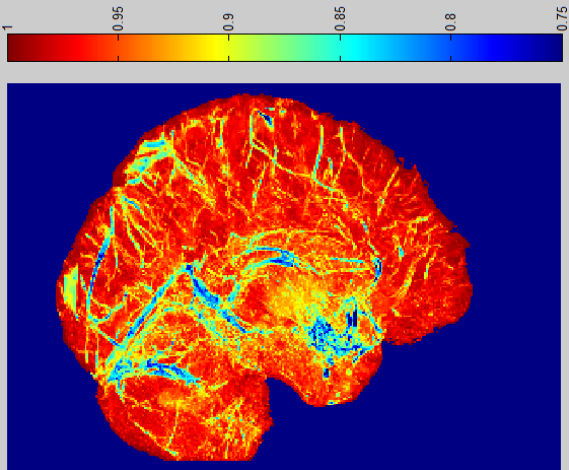
\includegraphics[width=9cm]{6_25_ex2}
\caption{Estimation de la SvO2 sur nos images issue de Figure 12. Les données viables sont situées dans les veines.}
\label{fig:6_25_ex2}	
\end{figure}


\bibliography{jeremythesebib}{}
\bibliographystyle{francaissc}